%%%%%%%%%%%%%%%%%%%%%%%%%%%%%%%%%%%%%%%%%
% The Legrand Orange Book
% LaTeX Template
% Version 2.1.1 (14/2/16)
%
% This template has been downloaded from:
% http://www.LaTeXTemplates.com
%
% Original author:
% Mathias Legrand (legrand.mathias@gmail.com) with modifications by:
% Vel (vel@latextemplates.com)
%
% License:
% CC BY-NC-SA 3.0 (http://creativecommons.org/licenses/by-nc-sa/3.0/)
%
% Compiling this template:
% This template uses biber for its bibliography and makeindex for its index.
% When you first open the template, compile it from the command line with the 
% commands below to make sure your LaTeX distribution is configured correctly:
%
% 1) pdflatex main
% 2) makeindex main.idx -s StyleInd.ist
% 3) biber main
% 4) pdflatex main x 2
%
% After this, when you wish to update the bibliography/index use the appropriate
% command above and make sure to compile with pdflatex several times 
% afterwards to propagate your changes to the document.
%
% This template also uses a number of packages which may need to be
% updated to the newest versions for the template to compile. It is strongly
% recommended you update your LaTeX distribution if you have any
% compilation errors.
%
% Important note:
% Chapter heading images should have a 2:1 width:height ratio,
% e.g. 920px width and 460px height.
%
%%%%%%%%%%%%%%%%%%%%%%%%%%%%%%%%%%%%%%%%%

%----------------------------------------------------------------------------------------
%	PACKAGES AND OTHER DOCUMENT CONFIGURATIONS
%----------------------------------------------------------------------------------------

\documentclass[11pt,fleqn]{book} % Default font size and left-justified equations

%----------------------------------------------------------------------------------------

%%%%%%%%%%%%%%%%%%%%%%%%%%%%%%%%%%%%%%%%%
% The Legrand Orange Book
% Structural Definitions File
% Version 2.0 (9/2/15)
%
% Original author:
% Mathias Legrand (legrand.mathias@gmail.com) with modifications by:
% Vel (vel@latextemplates.com)
% 
% This file has been downloaded from:
% http://www.LaTeXTemplates.com
%
% License:
% CC BY-NC-SA 3.0 (http://creativecommons.org/licenses/by-nc-sa/3.0/)
%
%%%%%%%%%%%%%%%%%%%%%%%%%%%%%%%%%%%%%%%%%

%----------------------------------------------------------------------------------------
%	VARIOUS REQUIRED PACKAGES AND CONFIGURATIONS
%----------------------------------------------------------------------------------------

\usepackage[top=3cm,bottom=3cm,left=3cm,right=3cm,headsep=10pt,a4paper]{geometry} % Page margins

\usepackage{graphicx} % Required for including pictures
\graphicspath{{Pictures/}} % Specifies the directory where pictures are stored

\usepackage{lipsum} % Inserts dummy text

\usepackage{tikz} % Required for drawing custom shapes
\usetikzlibrary{matrix}

\usepackage[english]{babel} % English language/hyphenation

\usepackage{enumitem} % Customize lists
\setlist{nolistsep} % Reduce spacing between bullet points and numbered lists

\usepackage{booktabs} % Required for nicer horizontal rules in tables

\usepackage{xcolor} % Required for specifying colors by name
\definecolor{ocre}{RGB}{243,102,25} % Define the orange color used for highlighting throughout the book

\usepackage{amssymb}
\usepackage{latexsym}
\usepackage{amsmath}
\usepackage{float}
\usepackage{ifpdf}
\usepackage{pgfplots}
\usepackage{xspace}




\input xy
\xyoption{all}



%-----------------------------
% USER DEFINED COMMANDS
%------------------------------
\newcommand{\mychaptername}{Chapter}
\allowdisplaybreaks

\usetikzlibrary{automata, positioning}


%----------------------------------------------------------------------------------------
%	FONTS
%----------------------------------------------------------------------------------------

\usepackage{avant} % Use the Avantgarde font for headings
%\usepackage{times} % Use the Times font for headings
%\usepackage{mathpazo} % Use the Palatino font for the default text. This prevents mathcal{} command from producing overly scripted letters.
\usepackage{mathptmx} % Use the Adobe Times Roman as the default text font together with math symbols from the Sym­bol, Chancery and Com­puter Modern fonts
\DeclareMathAlphabet{\mathcal}{OMS}{cmsy}{m}{n}

\usepackage{microtype} % Slightly tweak font spacing for aesthetics
\usepackage[utf8]{inputenc} % Required for including letters with accents
\usepackage[T1]{fontenc} % Use 8-bit encoding that has 256 glyphs

%----------------------------------------------------------------------------------------
%	BIBLIOGRAPHY AND INDEX
%----------------------------------------------------------------------------------------

\usepackage[style=alphabetic,citestyle=numeric,sorting=nyt,sortcites=true,autopunct=true,babel=hyphen,hyperref=true,abbreviate=false,backref=true,backend=biber]{biblatex}
\addbibresource{bibliography.bib} % BibTeX bibliography file
\defbibheading{bibempty}{}

\usepackage{calc} % For simpler calculation - used for spacing the index letter headings correctly
\usepackage{makeidx} % Required to make an index
\makeindex % Tells LaTeX to create the files required for indexing

%----------------------------------------------------------------------------------------
%	MAIN TABLE OF CONTENTS
%----------------------------------------------------------------------------------------

\usepackage{titletoc} % Required for manipulating the table of contents

\contentsmargin{0cm} % Removes the default margin

% Part text styling
\titlecontents{part}[0cm]
{\addvspace{20pt}\centering\large\bfseries}
{}
{}
{}

% Chapter text styling
\titlecontents{chapter}[1.25cm] % Indentation
{\addvspace{12pt}\large\sffamily\bfseries} % Spacing and font options for chapters
{\color{ocre!60}\contentslabel[\Large\thecontentslabel]{1.25cm}\color{ocre}} % Chapter number
{\color{ocre}}  
{\color{ocre!60}\normalsize\;\titlerule*[.5pc]{.}\;\thecontentspage} % Page number

% Section text styling
\titlecontents{section}[1.25cm] % Indentation
{\addvspace{3pt}\sffamily\bfseries} % Spacing and font options for sections
{\contentslabel[\thecontentslabel]{1.25cm}} % Section number
{}
{\hfill\color{black}\thecontentspage} % Page number
[]

% Subsection text styling
\titlecontents{subsection}[1.25cm] % Indentation
{\addvspace{1pt}\sffamily\small} % Spacing and font options for subsections
{\contentslabel[\thecontentslabel]{1.25cm}} % Subsection number
{}
{\ \titlerule*[.5pc]{.}\;\thecontentspage} % Page number
[]

% List of figures
\titlecontents{figure}[0em]
{\addvspace{-5pt}\sffamily}
{\thecontentslabel\hspace*{1em}}
{}
{\ \titlerule*[.5pc]{.}\;\thecontentspage}
[]

% List of tables
\titlecontents{table}[0em]
{\addvspace{-5pt}\sffamily}
{\thecontentslabel\hspace*{1em}}
{}
{\ \titlerule*[.5pc]{.}\;\thecontentspage}
[]

%----------------------------------------------------------------------------------------
%	MINI TABLE OF CONTENTS IN PART HEADS
%----------------------------------------------------------------------------------------

% Chapter text styling
\titlecontents{lchapter}[0em] % Indenting
{\addvspace{15pt}\large\sffamily\bfseries} % Spacing and font options for chapters
{\color{ocre}\contentslabel[\Large\thecontentslabel]{1.25cm}\color{ocre}} % Chapter number
{}  
{\color{ocre}\normalsize\sffamily\bfseries\;\titlerule*[.5pc]{.}\;\thecontentspage} % Page number

% Section text styling
\titlecontents{lsection}[0em] % Indenting
{\sffamily\small} % Spacing and font options for sections
{\contentslabel[\thecontentslabel]{1.25cm}} % Section number
{}
{}

% Subsection text styling
\titlecontents{lsubsection}[.5em] % Indentation
{\normalfont\footnotesize\sffamily} % Font settings
{}
{}
{}

%----------------------------------------------------------------------------------------
%	PAGE HEADERS
%----------------------------------------------------------------------------------------

\usepackage{fancyhdr} % Required for header and footer configuration

\pagestyle{fancy}
\renewcommand{\chaptermark}[1]{\markboth{\sffamily\normalsize\bfseries\mychaptername\ \thechapter:\ #1}{}} % Chapter text font settings
\renewcommand{\sectionmark}[1]{\markright{\sffamily\normalsize\thesection\hspace{5pt}#1}{}} % Section text font settings
\fancyhf{} \fancyhead[LE,RO]{\sffamily\normalsize\thepage} % Font setting for the page number in the header
\fancyhead[LO]{\rightmark} % Print the nearest section name on the left side of odd pages
\fancyhead[RE]{\leftmark} % Print the current chapter name on the right side of even pages
\renewcommand{\headrulewidth}{0.5pt} % Width of the rule under the header
\addtolength{\headheight}{2.5pt} % Increase the spacing around the header slightly
\renewcommand{\footrulewidth}{0pt} % Removes the rule in the footer
\fancypagestyle{plain}{\fancyhead{}\renewcommand{\headrulewidth}{0pt}} % Style for when a plain pagestyle is specified

% Removes the header from odd empty pages at the end of chapters
\makeatletter
\renewcommand{\cleardoublepage}{
\clearpage\ifodd\c@page\else
\hbox{}
\vspace*{\fill}
\thispagestyle{empty}
\newpage
\fi}

%----------------------------------------------------------------------------------------
%	THEOREM STYLES
%----------------------------------------------------------------------------------------

\usepackage{amsmath,amsfonts,amssymb,amsthm} % For math equations, theorems, symbols, etc

\newcommand{\intoo}[2]{\mathopen{]}#1\,;#2\mathclose{[}}
\newcommand{\ud}{\mathop{\mathrm{{}d}}\mathopen{}}
\newcommand{\intff}[2]{\mathopen{[}#1\,;#2\mathclose{]}}
\newtheorem{notation}{Notation}[chapter]

% Boxed/framed environments
\newtheoremstyle{ocrenumbox}% % Theorem style name
{0pt}% Space above
{0pt}% Space below
{\normalfont}% % Body font
{}% Indent amount
{\small\bf\sffamily\color{ocre}}% % Theorem head font
{\;}% Punctuation after theorem head
{0.25em}% Space after theorem head
{\small\sffamily\color{ocre}\thmname{#1}\nobreakspace\thmnumber{\@ifnotempty{#1}{}\@upn{#2}}% Theorem text (e.g. Theorem 2.1)
\thmnote{\nobreakspace\the\thm@notefont\sffamily\bfseries\color{black}---\nobreakspace#3.}} % Optional theorem note
\renewcommand{\qedsymbol}{$\blacksquare$}% Optional qed square

\newtheoremstyle{blacknumex}% Theorem style name
{5pt}% Space above
{5pt}% Space below
{\normalfont}% Body font
{} % Indent amount
{\small\bf\sffamily}% Theorem head font
{\;}% Punctuation after theorem head
{0.25em}% Space after theorem head
{\small\sffamily%{\tiny\ensuremath{\blacksquare}}
\nobreakspace\thmname{#1}\nobreakspace\thmnumber{\@ifnotempty{#1}{}\@upn{#2}}% Theorem text (e.g. Theorem 2.1)
\thmnote{\nobreakspace\the\thm@notefont\sffamily\bfseries---\nobreakspace#3.}}% Optional theorem note

\newtheoremstyle{blacknumbox} % Theorem style name
{0pt}% Space above
{0pt}% Space below
{\normalfont}% Body font
{}% Indent amount
{\small\bf\sffamily}% Theorem head font
{\;}% Punctuation after theorem head
{0.25em}% Space after theorem head
{\small\sffamily\thmname{#1}\nobreakspace\thmnumber{\@ifnotempty{#1}{}\@upn{#2}}% Theorem text (e.g. Theorem 2.1)
\thmnote{\nobreakspace\the\thm@notefont\sffamily\bfseries---\nobreakspace#3.}}% Optional theorem note

% Non-boxed/non-framed environments
\newtheoremstyle{ocrenum}% % Theorem style name
{5pt}% Space above
{5pt}% Space below
{\normalfont}% % Body font
{}% Indent amount
{\small\bf\sffamily\color{ocre}}% % Theorem head font
{\;}% Punctuation after theorem head
{0.25em}% Space after theorem head
{\small\sffamily\color{ocre}\thmname{#1}\nobreakspace\thmnumber{\@ifnotempty{#1}{}\@upn{#2}}% Theorem text (e.g. Theorem 2.1)
\thmnote{\nobreakspace\the\thm@notefont\sffamily\bfseries\color{black}---\nobreakspace#3.}} % Optional theorem note
\renewcommand{\qedsymbol}{$\blacksquare$}% Optional qed square
\makeatother

% Defines the theorem text style for each type of theorem to one of the three styles above
\newcounter{dummy} 
\numberwithin{dummy}{section}
\theoremstyle{ocrenumbox}
\newtheorem{theoremeT}[dummy]{Theorem}
\newtheorem{problem}[dummy]{Problem}
\newtheorem{exerciseT}[dummy]{Exercise}
\theoremstyle{blacknumex}
\newtheorem{exampleT}[dummy]{Example}
\theoremstyle{blacknumbox}
\newtheorem{vocabulary}[dummy]{Vocabulary}
\newtheorem{definitionT}[dummy]{Definition}
\newtheorem{corollaryT}[dummy]{Corollary}
\theoremstyle{ocrenum}
\newtheorem{propositionT}[dummy]{Proposition}

%----------------------------------------------------------------------------------------
%	DEFINITION OF COLORED BOXES
%----------------------------------------------------------------------------------------

\RequirePackage[framemethod=default]{mdframed} % Required for creating the theorem, definition, exercise and corollary boxes

% Theorem box
\newmdenv[skipabove=7pt,
skipbelow=7pt,
backgroundcolor=black!5,
linecolor=ocre,
innerleftmargin=5pt,
innerrightmargin=5pt,
innertopmargin=5pt,
leftmargin=0cm,
rightmargin=0cm,
innerbottommargin=5pt]{tBox}

% Exercise box	  
\newmdenv[skipabove=7pt,
skipbelow=7pt,
rightline=false,
leftline=true,
topline=false,
bottomline=false,
backgroundcolor=ocre!10,
linecolor=ocre,
innerleftmargin=5pt,
innerrightmargin=5pt,
innertopmargin=5pt,
innerbottommargin=5pt,
leftmargin=0cm,
rightmargin=0cm,
linewidth=4pt]{eBox}	

% Definition box
\newmdenv[skipabove=7pt,
skipbelow=7pt,
rightline=false,
leftline=true,
topline=false,
bottomline=false,
linecolor=ocre,
innerleftmargin=5pt,
innerrightmargin=5pt,
innertopmargin=0pt,
leftmargin=0cm,
rightmargin=0cm,
linewidth=4pt,
innerbottommargin=0pt]{dBox}	

% Corollary box
\newmdenv[skipabove=7pt,
skipbelow=7pt,
rightline=false,
leftline=true,
topline=false,
bottomline=false,
linecolor=gray,
backgroundcolor=black!5,
innerleftmargin=5pt,
innerrightmargin=5pt,
innertopmargin=5pt,
leftmargin=0cm,
rightmargin=0cm,
linewidth=4pt,
innerbottommargin=5pt]{cBox}

% Creates an environment for each type of theorem and assigns it a theorem text style from the "Theorem Styles" section above and a colored box from above
\newenvironment{theorem}{\begin{tBox}\begin{theoremeT}}{\end{theoremeT}\end{tBox}}
\newenvironment{proposition}{\begin{tBox}\begin{propositionT}}{\end{propositionT}\end{tBox}}
\newenvironment{exercise}{\begin{eBox}\begin{exerciseT}}{\hfill{\color{ocre}\tiny\ensuremath{\blacksquare}}\end{exerciseT}\end{eBox}}				  
\newenvironment{definition}{\begin{dBox}\begin{definitionT}}{\end{definitionT}\end{dBox}}	
\newenvironment{example}{\begin{cBox}\begin{exampleT}}{\end{exampleT}\end{cBox}}		
%\newenvironment{example}{\begin{cBox}\begin{exampleT}}%{\hfill{\tiny\ensuremath{\blacksquare}}
%{\end{exampleT}\end{cBox}}	
\newenvironment{corollary}{\begin{tBox}\begin{corollaryT}}{\end{corollaryT}\end{tBox}}	

%----------------------------------------------------------------------------------------
%	REMARK ENVIRONMENT
%----------------------------------------------------------------------------------------

\newenvironment{remark}{\par\vspace{10pt}\small % Vertical white space above the remark and smaller font size
\begin{list}{}{
\leftmargin=35pt % Indentation on the left
\rightmargin=25pt}\item\ignorespaces % Indentation on the right
\makebox[-2.5pt]{\begin{tikzpicture}[overlay]
\node[draw=ocre!60,line width=1pt,circle,fill=ocre!25,font=\sffamily\bfseries,inner sep=2pt,outer sep=0pt] at (-15pt,0pt){\textcolor{ocre}{R}};\end{tikzpicture}} % Orange R in a circle
\advance\baselineskip -1pt}{\end{list}\vskip5pt} % Tighter line spacing and white space after remark

%----------------------------------------------------------------------------------------
%	SECTION NUMBERING IN THE MARGIN
%----------------------------------------------------------------------------------------

\makeatletter
\renewcommand{\@seccntformat}[1]{\llap{\textcolor{ocre}{\csname the#1\endcsname}\hspace{1em}}}                    
\renewcommand{\section}{\@startsection{section}{1}{\z@}
{-4ex \@plus -1ex \@minus -.4ex}
{1ex \@plus.2ex }
{\normalfont\large\sffamily\bfseries}}
\renewcommand{\subsection}{\@startsection {subsection}{2}{\z@}
{-3ex \@plus -0.1ex \@minus -.4ex}
{0.5ex \@plus.2ex }
{\normalfont\sffamily\bfseries}}
\renewcommand{\subsubsection}{\@startsection {subsubsection}{3}{\z@}
{-2ex \@plus -0.1ex \@minus -.2ex}
{.2ex \@plus.2ex }
{\normalfont\small\sffamily\bfseries}}                        
\renewcommand\paragraph{\@startsection{paragraph}{4}{\z@}
{-2ex \@plus-.2ex \@minus .2ex}
{.1ex}
{\normalfont\small\sffamily\bfseries}}

%----------------------------------------------------------------------------------------
%	PART HEADINGS
%----------------------------------------------------------------------------------------

% numbered part in the table of contents
\newcommand{\@mypartnumtocformat}[2]{%
\setlength\fboxsep{0pt}%
\noindent\colorbox{ocre!20}{\strut\parbox[c][.7cm]{\ecart}{\color{ocre!70}\Large\sffamily\bfseries\centering#1}}\hskip\esp\colorbox{ocre!40}{\strut\parbox[c][.7cm]{\linewidth-\ecart-\esp}{\Large\sffamily\centering#2}}}%
%%%%%%%%%%%%%%%%%%%%%%%%%%%%%%%%%%
% unnumbered part in the table of contents
\newcommand{\@myparttocformat}[1]{%
\setlength\fboxsep{0pt}%
\noindent\colorbox{ocre!40}{\strut\parbox[c][.7cm]{\linewidth}{\Large\sffamily\centering#1}}}%
%%%%%%%%%%%%%%%%%%%%%%%%%%%%%%%%%%
\newlength\esp
\setlength\esp{4pt}
\newlength\ecart
\setlength\ecart{1.2cm-\esp}
\newcommand{\thepartimage}{}%
\newcommand{\partimage}[1]{\renewcommand{\thepartimage}{#1}}%
\def\@part[#1]#2{%
\ifnum \c@secnumdepth >-2\relax%
\refstepcounter{part}%
\addcontentsline{toc}{part}{\texorpdfstring{\protect\@mypartnumtocformat{\thepart}{#1}}{\partname~\thepart\ ---\ #1}}
\else%
\addcontentsline{toc}{part}{\texorpdfstring{\protect\@myparttocformat{#1}}{#1}}%
\fi%
\startcontents%
\markboth{}{}%
{\thispagestyle{empty}%
\begin{tikzpicture}[remember picture,overlay]%
\node at (current page.north west){\begin{tikzpicture}[remember picture,overlay]%	
\fill[ocre!20](0cm,0cm) rectangle (\paperwidth,-\paperheight);
\node[anchor=north] at (4cm,-3.25cm){\color{ocre!40}\fontsize{220}{100}\sffamily\bfseries\@Roman\c@part}; 
\node[anchor=south east] at (\paperwidth-1cm,-\paperheight+1cm){\parbox[t][][t]{8.5cm}{
\printcontents{l}{0}{\setcounter{tocdepth}{1}}%
}};
\node[anchor=north east] at (\paperwidth-1.5cm,-3.25cm){\parbox[t][][t]{15cm}{\strut\raggedleft\color{white}\fontsize{30}{30}\sffamily\bfseries#2}};
\end{tikzpicture}};
\end{tikzpicture}}%
\@endpart}
\def\@spart#1{%
\startcontents%
\phantomsection
{\thispagestyle{empty}%
\begin{tikzpicture}[remember picture,overlay]%
\node at (current page.north west){\begin{tikzpicture}[remember picture,overlay]%	
\fill[ocre!20](0cm,0cm) rectangle (\paperwidth,-\paperheight);
\node[anchor=north east] at (\paperwidth-1.5cm,-3.25cm){\parbox[t][][t]{15cm}{\strut\raggedleft\color{white}\fontsize{30}{30}\sffamily\bfseries#1}};
\end{tikzpicture}};
\end{tikzpicture}}
\addcontentsline{toc}{part}{\texorpdfstring{%
\setlength\fboxsep{0pt}%
\noindent\protect\colorbox{ocre!40}{\strut\protect\parbox[c][.7cm]{\linewidth}{\Large\sffamily\protect\centering #1\quad\mbox{}}}}{#1}}%
\@endpart}
\def\@endpart{\vfil\newpage
\if@twoside
\if@openright
\null
\thispagestyle{empty}%
\newpage
\fi
\fi
\if@tempswa
\twocolumn
\fi}

%----------------------------------------------------------------------------------------
%	CHAPTER HEADINGS
%----------------------------------------------------------------------------------------

% A switch to conditionally include a picture, implemented by  Christian Hupfer
\newif\ifusechapterimage
\usechapterimagetrue
\newcommand{\thechapterimage}{}%
\newcommand{\chapterimage}[1]{\ifusechapterimage\renewcommand{\thechapterimage}{#1}\fi}%
\def\@makechapterhead#1{%
{\parindent \z@ \raggedright \normalfont
\ifnum \c@secnumdepth >\m@ne
\if@mainmatter
\begin{tikzpicture}[remember picture,overlay]
\node at (current page.north west)
{\begin{tikzpicture}[remember picture,overlay]
\node[anchor=north west,inner sep=0pt] at (0,0) {\ifusechapterimage\includegraphics[width=\paperwidth]{\thechapterimage}\fi};
\draw[anchor=west] (\Gm@lmargin,-9cm) node [line width=2pt,rounded corners=15pt,draw=ocre,fill=white,fill opacity=0.5,inner sep=15pt]{\strut\makebox[22cm]{}};
\draw[anchor=west] (\Gm@lmargin+.3cm,-9cm) node {\huge\sffamily\bfseries\color{black} \mychaptername{} \thechapter: #1\strut};
\end{tikzpicture}};
\end{tikzpicture}
\else
\begin{tikzpicture}[remember picture,overlay]
\node at (current page.north west)
{\begin{tikzpicture}[remember picture,overlay]
\node[anchor=north west,inner sep=0pt] at (0,0) {\ifusechapterimage\includegraphics[width=\paperwidth]{\thechapterimage}\fi};
\draw[anchor=west] (\Gm@lmargin,-9cm) node [line width=2pt,rounded corners=15pt,draw=ocre,fill=white,fill opacity=0.5,inner sep=15pt]{\strut\makebox[22cm]{}};
\draw[anchor=west] (\Gm@lmargin+.3cm,-9cm) node {\huge\sffamily\bfseries\color{black}#1\strut};
\end{tikzpicture}};
\end{tikzpicture}
\fi\fi\par\vspace*{270\p@}}}

%-------------------------------------------

\def\@makeschapterhead#1{%
\begin{tikzpicture}[remember picture,overlay]
\node at (current page.north west)
{\begin{tikzpicture}[remember picture,overlay]
\node[anchor=north west,inner sep=0pt] at (0,0) {\ifusechapterimage\includegraphics[width=\paperwidth]{\thechapterimage}\fi};
\draw[anchor=west] (\Gm@lmargin,-9cm) node [line width=2pt,rounded corners=15pt,draw=ocre,fill=white,fill opacity=0.5,inner sep=15pt]{\strut\makebox[22cm]{}};
\draw[anchor=west] (\Gm@lmargin+.3cm,-9cm) node {\huge\sffamily\bfseries\color{black}#1\strut};
\end{tikzpicture}};
\end{tikzpicture}
\par\vspace*{270\p@}}
\makeatother

%----------------------------------------------------------------------------------------
%	HYPERLINKS IN THE DOCUMENTS
%----------------------------------------------------------------------------------------

\usepackage{hyperref}
\hypersetup{hidelinks,backref=true,pagebackref=true,hyperindex=true,colorlinks=true,breaklinks=true,urlcolor= ocre,linkcolor=ocre,bookmarks=true,bookmarksopen=false,pdftitle={Information Theory},pdfauthor={Yfke Dulek, Christian Schaffner}}
\usepackage{bookmark}
\bookmarksetup{
open,
numbered,
addtohook={%
\ifnum\bookmarkget{level}=0 % chapter
\bookmarksetup{bold}%
\fi
\ifnum\bookmarkget{level}=-1 % part
\bookmarksetup{color=ocre,bold}%
\fi
}
}



%---------------------------------------
%     USER DEFINED COMMANDS
%---------------------------------------
\newcommand{\term}[1]{{\small\bf\sffamily{#1}\normalfont}}
\newcommand{\chris}[1]{{ \color{blue} [{\bf Chris:} #1] }}
\newcommand{\yfke}[1]{{ \color{red} [{\bf Yfke:} #1] }}
 % Insert the commands.tex file which contains the majority of the structure behind the template

\tikzset{
  marked/.style      = {circle,draw,inner sep=1.75,color=ocre,fill=ocre},
  dummy/.style    = {circle,draw,inner sep=0.5,fill=black}
}

\begin{document}

\newcommand{\CF}{\href{https://www.cwi.nl/crypto/docs/InfTheory2.pdf}{[CF]}}
\newcommand{\CT}{\href{http://onlinelibrary.wiley.com/book/10.1002/0471200611}{[CT]}}

%----------------------------------------------------------------------------------------
%	TITLE PAGE
%----------------------------------------------------------------------------------------

\begingroup
\thispagestyle{empty}
\begin{tikzpicture}[remember picture,overlay]
\coordinate [below=12cm] (midpoint) at (current page.north);
\node at (current page.north west)
{\begin{tikzpicture}[remember picture,overlay]
%%\node[anchor=north west,inner sep=0pt] at (0,0) {\includegraphics[width=\paperwidth]{background}}; % Background image
\draw[anchor=north] (midpoint) node [fill=ocre!30!white,fill opacity=0.6,text opacity=1,inner sep=1cm]{\Huge\centering\bfseries\sffamily\parbox[c][][t]{\paperwidth}{\centering Information Theory\\[15pt] % Book title
{\Large University of Amsterdam, \href{https://www.illc.uva.nl/MScLogic/}{Master of Logic}, Fall 2016}\\[20pt] % Subtitle
{\Large Yfke Dulek and Christian Schaffner}}}; % Author name
\end{tikzpicture}};
\end{tikzpicture}
\vfill
{\small \noindent 

}
\endgroup

%----------------------------------------------------------------------------------------
%	COPYRIGHT PAGE
%----------------------------------------------------------------------------------------

\newpage
~\vfill
\thispagestyle{empty}

\noindent Copyright \copyright\ 2016 Yfke Dulek and Christian Schaffner\\ % Copyright notice

\noindent These lecture notes are licenced under the \href{https://creativecommons.org/licenses/by-nc-sa/4.0/}{Creative Commons Attribution-NonCommercial-ShareAlike 4.0 International} license.\\

The source is available on \href{https://github.com/cschaffner/InformationTheory}{github} and we are grateful for any feedback including typos and suggestions for improvements! Feel free to send us \href{https://help.github.com/articles/about-pull-requests/}{pull requests}.\\


% \noindent \textsc{Published by Publisher}\\ % Publisher

% \noindent \textsc{Source}\\ % URL

\noindent Parts of the text is based on, or taken verbatim, from `The Mathematical Theory of Information, and Applications' (version 2.0) by Ronald Cramer and Serge Fehr \CF. The lay-out is based on the Legrand Orange Book (version 2.1.1), licenced under the \href{https://creativecommons.org/licenses/by-nc-sa/3.0/}{Creative Commons License BY-NC-SA 3.0}.\\

% Unless required by applicable law or agreed to in writing, software distributed under the License is distributed on an \textsc{``as is'' basis, without warranties or conditions of any kind}, either express or implied. See the License for the specific language governing permissions and limitations under the License.\\ % License information

% \noindent \textit{First printing, March 2013} % Printing/edition date

%----------------------------------------------------------------------------------------
%	TABLE OF CONTENTS
%----------------------------------------------------------------------------------------

\usechapterimagefalse % If you don't want to include a chapter image, use this to toggle images off - it can be enabled later with \usechapterimagetrue

%\chapterimage{chapter_head_1.pdf} % Table of contents heading image

\pagestyle{empty} % No headers

\tableofcontents % Print the table of contents itself

\cleardoublepage % Forces the first chapter to start on an odd page so it's on the right

\pagestyle{fancy} % Print headers again

%-----------------------------
%ACTUAL CONTENT
%-----------------------------



%Sets
\newcommand{\N}{\mathbb{N}}
\newcommand{\R}{\mathbb{R}}
\newcommand{\im}{\mathrm{im}}
\newcommand{\set}[1]{\{#1\}}
\newcommand{\Set}[2]{\{#1\,|\,#2\}}
\newcommand{\SET}[3][\big]{#1\{#2\,#1|\,#3#1\}}

%Events
\newcommand{\evA}{\mathcal{A}}
\newcommand{\evB}{\mathcal{B}}


\newcommand{\es}{\bot}
\newcommand{\strg}{\{0,1\}^*}
\newcommand{\len}{\ell}

\newcommand{\col}{\mathrm{Col}}
\newcommand{\guess}{{\sl guess}}

\newcommand{\bfX}{\text{\boldmath $X$}}
\newcommand{\bfx}{\text{\boldmath $x$}}

\newcommand{\AC}{A\hspace{-0.2ex}C}

\newcommand{\supp}{\mathrm{supp}}
\newcommand{\Exp}{\mathbb{E}}
\newcommand{\Var}{\mathrm{Var}}


\newcommand{\entropydiagramXY}[7][1.5]{
\begin{tikzpicture}
\def\size{#1}
\draw (0,0) circle (\size cm);
\draw (\size,0) circle (\size cm);
\node at (-\size/2,0) {#5};
\node at (\size+\size/2,0) {#6};
\node at (\size/2,0) {#7};
\node at (\size/2,-\size - 0.25*\size) {#4};
\node at (-\size/2,\size + 0.1) {#2};
\node at (\size*1.5,\size + 0.1) {#3};
\end{tikzpicture}
}

\newcommand{\entropydiagramXYZ}[7][1.5]{
\begin{tikzpicture}
\def\size{#1}
\draw (0,0) circle (\size cm);
\draw (\size,0) circle (\size cm);
\draw (\size/2,-\size) circle (\size cm);
\node at (-\size/2,0) {#5};
\node at (\size+\size/2,0) {#6};
\node at (\size/2,0) {#7};
\node at (\size/2,-\size - 0.25*\size) {#4};
\node at (-\size/2,\size + 0.1) {#2};
\node at (\size*1.5,\size + 0.1) {#3};
\end{tikzpicture}
}


%\chapter*{Introduction}
%This is an introduction to the IT course. Lecture notes are based on the CF script. Copy introduction from there? The template is under a creative commons license, so we should probably have some attribution to them.
%
%We could also publish the intro only on moodle, and publish each week's content as separate files.




\chapter{Probability and Entropy}
\setcounter{page}{1}
\section{Preliminaries: Probability Theory}
For this course, we will only be concerned with discrete probabilities. This section formalizes some notions you should already be familiar with: probability spaces, events and probability distributions.

\begin{definition}[Probability space]
A (discrete) probability space $(\Omega, \mathcal{F}, P)$ consists of a
discrete, non-empty \emph{sample space} $\Omega$, an \emph{event space}
$\mathcal{F} \subseteq \mathcal{P}(\Omega)$ and a \emph{probability measure} $P$ which is a function $P : \Omega \to \R_{\geq 0}$ that satisfies
\[
\sum_{\omega \in \Omega} P(\omega) = 1.
\]
\end{definition}
The event space $\mathcal{F}$ is required to be non-empty and closed under
intersection, union and complements. For convenience, we will most
often assume that $\mathcal{F}$ equals the powerset
$\mathcal{P}(\Omega)$ of $\Omega$, i.e.\ it
contains all
possible subsets of events, and therefore fulfils the required properties.

\begin{definition}[Event]\label{def:event}
An event $\evA$ is an element of the event space $\mathcal{F}
\subseteq \mathcal{P}(\Omega)$, i.e.\ a subset $\evA$ of the sample space $\Omega$. Its probability is defined as
\[
P[\evA] := \sum_{\omega \in \evA} P(\omega),
\]
where by convention $P[\emptyset] = 0$.
\end{definition}
As a notational convention, we write $P[\evA,\evB]$ for $P[\evA \cap \evB]$, and $P[\overline\evA]$ for $P[\Omega\backslash\evA]$.

\begin{exercise}
Prove the following identities (for arbitrary events $\evA, \evB \subseteq \Omega$):
\setlength{\abovedisplayskip}{0pt}
\setlength{\belowdisplayskip}{0pt}
\setlength{\abovedisplayshortskip}{0pt}
\setlength{\belowdisplayshortskip}{0pt}
\begin{align}
P[\overline{\evA}] &= 1 - P[\evA]\\
P[\evA \cup \evB] &= P[\evA] + P[\evB] - P[\evA, \evB]\\
P[\evA] &= P[\evA, \evB] + P[\evA, \overline\evB].
\end{align}
\end{exercise}
It is often useful to consider the probability of an event \emph{given} that some other event happened:
\begin{definition}[Conditional probability]\label{def:conditional-probability}
For events $\evA$ and $\evB$ with $P[\evA] > 0$, the conditional probability of $\evB$ given $\evA$ is defined as
\[
P[\evB | \evA] := \frac{P[\evA,\evB]}{P[\evA]} \, .
\]
\end{definition}
\begin{example}[Fair die]\label{ex:fair-die}
We throw a six-sided fair die once, and consider the number that comes
up. The sample space for this experiment is $\Omega =
\set{1,2,3,4,5,6}$, with event space $\mathcal{F} = \mathcal{P}(\Omega)$ and probability measure $P[i] =
\frac{1}{|\Omega|} = \frac{1}{6}$ for all $i \in \Omega$ (this is a
\term{uniform} probability measure). Consider the events $\evA = \set{2,4,6}$ and $\evB = \set{3,6}$.
Using the formulas in Definitions~\ref{def:event} and~\ref{def:conditional-probability}, we can compute the following probabilities:
\begin{align*}
P[\evA] &= \frac{1}{2} &\mbox{(the outcome is even)}\\
P[\evB] &= \frac{1}{3}&\mbox{(the outcome is a multiple of 3)}\\
P[\evA, \evB] &= P[\set{6}] = \frac{1}{6} & \mbox{(the roll is even \emph{and} a multiple of 3)}\\
P[\evA | \evB] &= \frac{1/6}{1/3} = \frac{1}{2} & \mbox{(the roll is even, \emph{given} that it is a multiple of 3)}\\
P[\evB | \evA] &= \frac{1/6}{1/2} = \frac{1}{3}& \mbox{(the roll is a multiple of 3, \emph{given} that it is even)}\\
\end{align*}
This example shows that in general, $P[\evA | \evB]$ is \emph{not
  equal} to $P[\evB | \evA]$.
\end{example}

\begin{definition}[(Discrete Random Variable (RV)]
Let $(\Omega, \mathcal{F}, P)$ be a discrete probability space. A
random variable $X$ is a function $X : \Omega \to \mathcal{X}$ where
$\mathcal{X}$ is a set, and we may assume it to be discrete.
\end{definition}
A \emph{real} random variable is one whose image is contained in $\mathbb{R}$. A (The \emph{image} and the \emph{range} of a random variable $X$ are given by the image and the range of $X$ in the function-theoretic sense.) The image of a \emph{binary} random variable is a set $\set{x_0, x_1}$ with only two elements.

\begin{definition}[Probability distribution]
Let $X$ be a random variable. The probability distribution of $X$ is the function $P_X : \mathcal{X} \to [0,1]$ defined as
\[
P_X(x) := P[X = x],
\]
where $X = x$ denotes the event $\Set{\omega \in \Omega}{X(\omega) = x}$.
\end{definition}
Alternatively, one can write $P_X(x) = P(X^{-1}(x))$ to express that the
probability of $x$ is precisely the $P$-measure of the pre-image of $x$
under the random variable $X$.

\begin{exercise}
Verify that $(\mathcal{X},
\mathcal{P}(\mathcal{X}), P_X)$ is itself a probability space.
\end{exercise}

We say that $P_X$ is a \term{uniform} distribution if the associated
probability measure is uniform, i.e. $P_X(x) =
\frac{1}{|\mathcal{X}|}$. The \term{support} of a random variable or a
probability distribution is
defined as $\supp(P_X) := \{x \in \mathcal{X} \mid P_X(x) > 0\}$, the
points of the range which have strictly positive probability. We often
slightly abuse notation and write $\supp(X)$ instead.

When given two or more random variables defined on the same probability space, we can consider the probability that each of the variables take on a certain value:

\begin{definition}[Joint probability distribution]
Let $X$ and $Y$ be two random variables defined on the same probability space, with respective ranges $\mathcal{X}$ and $\mathcal{Y}$. The pair $XY$ is a random variable with probability distribution $P_{XY} : \mathcal{X} \times \mathcal{Y} \to [0,1]$ given by
\[
P_{XY}(x,y) := P[X = x, Y = y].
\]
\end{definition}
This definition naturally extends to three and more random variables. Unless otherwise stated, a collection of random variables is assumed to be defined on the same (implicit) probability space, so that their joint distribution is always well-defined.

If $P_{XY} = P_X \cdot P_Y$, in the sense that $P_{XY}(x,y) = P_X(x)P_Y(y)$ for all $x \in \mathcal{X}$ and $y 
\in \mathcal{Y}$, then the random variables $X$ and $Y$ are said to be \term{independent}. If a set of variables $X_1, ..., X_n$ are all mutually independent and all have the same distribution (i.e. $P_{X_i} = P_{X_j}$ for all $i,j$), then they are \term{independent and identically distributed}, or \term{i.i.d.}

From a joint distribution, we can always find out the ``original'' (or \term{marginal}) distribution of one of the random variables (for example, $X$) by \term{marginalizing} out the variable that we want to discard (for example, $Y$):
\begin{align}
P_X(x) = \sum_{y \in \mathcal{Y}} P_{XY}(x,y).
\end{align}
This marginalization process also works with more than two random variables.

Like events, probability distributions can also be conditioned on
probabilistic events:
\begin{definition}[Conditional probability distribution]
If $\evA$ is an event with $P[\evA] > 0$, then the conditional probability distribution of $X$ given $\evA$ is given by
\[
P_{X|\evA}(x) = \frac{P[X=x, \evA]}{P[\evA]}.
\]
If $Y$ is another random variable and $P_Y(y) > 0$, then we write
\[
P_{X | Y}(x| y) := P_{X | Y = y}(x) = \frac{P_{XY}(x,y)}{P_Y(y)}
\]
for the conditional distribution of $X$, given $Y = y$.
\end{definition}
Note that again, both $(\mathcal{X},P_{X | \evA})$ and $(\mathcal{X},P_{X| Y=y})$ themselves form probability spaces. Note also that if $X$ and $Y$ are independent, then
\begin{align}
P_{X | Y}(x |y) = \frac{P_{XY}(x,y)}{P_Y(y)} = \frac{P_X(x) \cdot P_Y(y)}{P_Y(y)} = P_X(x),
\end{align}
which aligns well with our intuition of independent variables: the distribution of $X$ remains unchanged when $Y$ is fixed to a specific value.

\begin{example}[Fair die (continued)]
Consider again the throw of a six-sided fair die as in Example~\ref{ex:fair-die}. Let the random variable $X$ describe the number of integer divisors for the outcome, that is
\[X(1) = 1 \ \ \ \ \ X(2) = 2 \ \ \ \ \ X(3) = 2 \ \ \ \ \ X(4) = 3 \ \ \ \ \ X(5) = 2 \ \ \ \ \ X(6) = 3
\]
$X$ is a real random variable, with range $\mathcal{X} = \set{1,2,3}$. The associated probability distribution is
\[P_X(1) = P[\set{1}] = \frac{1}{6}, \ \ \ \ \ \ \ \ \ \ P_X(2) = P[\set{2,3,5}] = \frac{1}{2}, \ \ \ \ \ \ \ \ \ \ P_X(3) = P[\set{4,6}] = \frac{1}{3}.
\]
If we now condition on the event $\evA = \set{2,4,6}$ (the outcome being even), we get that
\[P_{X | \evA}(1) = 0, \ \ \ \ \ \ \ \ \ \ P_{X | \evA}(2) = \frac{1}{3}, \ \ \ \ \ \ \ \ \ \ P_{X | \evA}(3) = \frac{2}{3}.
\]
\end{example}
If $X$ is a random variable and $f : \mathcal{X} \to \mathcal{Y}$ is a surjective function, then $f(X)$ is a random variable, defined by composing the map $f$ with the map $X$. Its image is $\mathcal{Y}$. Clearly,
\[
P_{f(X)}(y) = \sum_{x \in \mathcal{X} : f(x) = y} P_X(x).
\]
For example, $1/P_X(X)$ denotes the real random variable obtained from another random variable $X$ by composing with the map $1/P_X$ that assigns $1/P_X(x) \in \mathbb{R}$ to $x \in \mathcal{X}$.

\begin{definition}[Expectation]
The expectation of a \emph{real} random variable $X$ is defined as
\[
\Exp[X] := \sum_{x \in \mathcal{X}} P_X(x) \cdot x.
\]
\end{definition}
Note that if $X$ is not real, then we can still consider the expectation of some function $f : \mathcal{X} \to \mathbb{R}$, where
\[
\Exp[f(X)] = \sum_{x \in \mathcal{X}} P_X(x) \cdot f(X).
\]
\begin{definition}[Variance]
The variance of a \emph{real} random variable $X$ is defined as
\[
\Var[X] := \Exp[(X - \Exp[X])^2].
\]
\end{definition}
The variation is a measure for the deviation of the mean. Hoeffding's inequality (here stated for binary random variables) states that for a list of i.i.d. random variables, the average of the random variables is close to the expectation, except with very small probability. We state it here without proof.

\begin{theorem}[Hoeffding's inequality]
Let $X_1, ..., X_n$ be independent and identically distributed binary random variables with $P_{X_i}(0) = 1 - \mu$ and $P_{X_i}(1) = \mu$, and thus $\Exp[X_i] = \mu$. Then, for any $\delta > 0$
\[
P\left[\sum_i X_i > (\mu + \delta) \cdot n\right] \leq \exp(-2\delta^2n).
\]
\end{theorem}

\section{Some Important Distributions}
\begin{itemize}
\item
The distribution of a biased coin with probability $P_X(1)=p$ to land
heads, and a probability of $P_X(0)=1-p$ to land tails is called
\href{https://en.wikipedia.org/wiki/Bernoulli_distribution}{\term{Bernoulli($p$)} distribution}. Its entropy is given by the binary
entropy $h(p)$. The expected value is $\Exp[X]=p$ and the variance is
$\Var[X]=p(1-p)$.
\item
When $n$ coins $X_1, X_2, \ldots, X_n$ are flipped independently and
every $X_i$ is Bernoulli($p$) distributed, let $S=\sum_{i=1}^n X_i$ be
their sum, i.e.\ the number of heads in $n$ throws of a biased
coin. Then, $S$ has the \href{https://en.wikipedia.org/wiki/Binomial_distribution}{\term{Binomial($n,p$)} distribution}:
\[
P_S(k) = \binom{n}{k} p^k (1-p)^{n-k} \mbox{ where } k=0,1,2,\ldots,n
\, .
\] 
From simple properties of the expected value and variance, one can
show that $\Exp[S]=np$ and $\Var[S]=np(1-p)$.
\item
The
\href{https://en.wikipedia.org/wiki/Geometric_distribution}{\term{Geometric($p$)}
  distribution} of a random variable $Y$ is defined as the number of
times one has to flip a Bernoulli($p$) coin before it lands heads:
\[ P_Y(k) = (1-p)^{k-1} p \mbox{ where } k=1,2,3,\ldots \, .
\]
There is another variant of the geometric distribution used in the literature,
where one excludes the final success event of landing
heads in the counting:
\[
P_Z(k) = (1-p)^k p \,  \mbox{ where } k=0,1,2,3,\ldots \, .
\] 
While the expected values are slightly different, namely
$\Exp[Y]=\frac{1}{p}$ and $\Exp[Z]=\frac{1-p}{p}$, their variances are
the same $\Var[Y]=\Var[Z]=\frac{1-p}{p^2}$.
\end{itemize}

\section{Jensen's Inequality}
In the following, let $\mathcal{D}$ be an interval in $\mathbb{R}$.

\begin{definition}[Convex and concave functions]
The function $f : \mathcal{D} \to \mathbb{R}$ is convex if for all $x_1, x_2 \in \mathcal{D}$ and all $\lambda \in [0,1] \subset \mathbb{R}$:
\[
\lambda f(x_1) + (1-\lambda)f(x_2) \geq f(\lambda x_1 + (1-\lambda)x_2).
\]
The function $f$ is \emph{strictly} convex if equality only holds when $\lambda \in \set{0,1}$ or when $x_1 = x_2$.
\\The function $f$ is (strictly) concave if the function $-f$ is (strictly) convex.
\end{definition}
Intuitively, a function is convex if any straight line drawn between two points $f(x_1)$ and $f(x_2)$ lies above the graph of $f$ entirely. For a concave function, such a line must lie entirely beneath the graph.
\begin{example}
The following functions are convex (for $c \in \mathbb{R}$):
\\
{
\centering
\begin{tabular}{ccccc}
\begin{tikzpicture}
	\begin{axis}[xmin=-2, xmax=2,ymin=0,ymax=2, ,axis x line=bottom, axis y line=center,ticks=none, x axis line style =-, y axis line style=-,width=4cm,height=3cm]
	\addplot[mark=none,domain=-2:2,color=ocre] {x^2};
	\end{axis}
\end{tikzpicture}%
	&
\begin{tikzpicture}
	\begin{axis}[xmin=-5, xmax=5,ymin=0,ymax=5, ,axis x line=bottom, axis y line=center,ticks=none, x axis line style =-, y axis line style=-,width=4cm,height=3cm]
	\addplot[mark=none,domain=-5:5,color=ocre] {exp(-x)};
	\end{axis}
\end{tikzpicture}%
	&
\begin{tikzpicture}
	\begin{axis}[xmin=0, xmax=3,ymin=-1.5,ymax=2, ,axis x line=center, axis y line=left,ticks=none, x axis line style =-, y axis line style=-,width=4cm,height=3cm]
	\addplot[mark=none,domain=0:5,color=ocre] {ln(1/x)/ln(2)};
	\end{axis}
\end{tikzpicture}%
	&
\begin{tikzpicture}
	\begin{axis}[xmin=0, xmax=3,ymin=-1.5,ymax=2, ,axis x line=center, axis y line=left,ticks=none, x axis line style =-, y axis line style=-,width=4cm,height=3cm]
	\addplot[mark=none,domain=0:5,color=ocre] {x*ln(x)/ln(2)};
	\end{axis}
\end{tikzpicture}%
	&
\begin{tikzpicture}
	\begin{axis}[xmin=0, xmax=3,ymin=0,ymax=2, ,axis x line=bottom, axis y line=center,ticks=none, x axis line style =-, y axis line style=-,width=4cm,height=3cm]
	\addplot[mark=none,domain=0:5,color=ocre] {1};
	\end{axis}
\end{tikzpicture}
	\\
	$x^2$ & $e^{-x}$ & $\log(1/x)$ & $x\cdot\log x$ & $c$\\
\end{tabular}
}
\\\\The following functions are concave (for $c \in \mathbb{R}$):\\
{
\centering
\begin{tabular}{ccc}
\begin{tikzpicture}
	\begin{axis}[xmin=0, xmax=3,ymin=-2,ymax=2, ,axis x line=center, axis y line=left,ticks=none, x axis line style =-, y axis line style=-,width=4cm,height=3cm]
	\addplot[mark=none,domain=0:5,color=ocre] {ln(x)/ln(2)};
	\end{axis}
\end{tikzpicture}%
	&
\begin{tikzpicture}
	\begin{axis}[xmin=0, xmax=3,ymin=0,ymax=2, ,axis x line=center, axis y line=left,ticks=none, x axis line style =-, y axis line style=-,width=4cm,height=3cm]
	\addplot[mark=none,domain=0:5,color=ocre] {sqrt(x)};
	\end{axis}
\end{tikzpicture}%
	&
\begin{tikzpicture}
	\begin{axis}[xmin=0, xmax=3,ymin=0,ymax=2, ,axis x line=bottom, axis y line=center,ticks=none, x axis line style =-, y axis line style=-,width=4cm,height=3cm]
	\addplot[mark=none,domain=0:5,color=ocre] {1};
	\end{axis}
\end{tikzpicture}
	\\
	$\log x$ & $\sqrt{x}$ & $c$\\
\end{tabular}
}
\end{example}
The following establishes a more formal method of proving the convexity of a function.
\begin{proposition}
Let $f : \mathcal{D} \to \mathbb{R}$. If $\mathcal{D}$ is open, and for all $x \in \mathcal{D}$, the second order derivative $f''(x)$ exists and is non-negative (positive), then $f$ is convex (strictly convex).
\end{proposition}
We omit the proof, which can be found in, for example, \href{http://homepages.cwi.nl/~schaffne/courses/inftheory/2016/notes/CramerFehr.pdf}{[CF]} (Lemma 1).


\begin{theorem}[Jensen's inequality] Let $f : \mathcal{D} \to \mathbb{R}$ be a convex function, and let $n \in \mathbb{N}$. Then for any $p_1, ..., p_n \in \mathbb{R}_{\geq 0}$ such that $\sum_{i=1}^n p_i = 1$ and for any $x_1, ..., x_n \in \mathcal{D}$ it holds that
\[
\sum_{i=1}^n p_if(x_i) \geq f\left(\sum_{i=1}^np_ix_i\right).
\]
If $f$ is strictly convex and $p_1, ..., p_n > 0$, then equality holds iff $x_1 = \cdots = x_n$.

In particular, if $X$ is a real random variable whose image $\mathcal{X}$ is contained in $\mathcal{D}$, then
\[
\Exp[f(X)] \geq f(\Exp[X]),
\]
and if $f$ is strictly convex, equality holds iff there is a $c \in \mathcal{X}$ such that $X = c$ with probability 1.
\end{theorem}
\begin{proof}
The proof is by induction. The case $n=1$ is trivial, and the case $n=2$ is identical to the very definition of convexity. Suppose that we have already proved the claim up to $n-1 \geq 2$. Assume, without loss of generality, that $p_n < 1$. Then:
\begin{align}
\sum_{i=1}^n p_i f(x_i) &= p_n f(x_n) + \sum_{i=1}^{n-1} p_i f(x_i)\nonumber\\
&= p_n f(x_n) + (1-p_n)\sum_{i=1}^{n-1} \frac{p_i}{1-p_n} f(x_i)\nonumber\\
&\geq p_n f(x_n) + (1-p_n)f\left(\sum_{i=1}^{n-1} \frac{p_i}{1-p_n} x_i\right) & \mbox{(induction hypothesis)}\nonumber\\
&\geq f\left(p_n x_n + (1-p_n)\sum_{i=1}^{n-1} \frac{p_i}{1-p_n} x_i\right) & \mbox{(definition of convexity)}\nonumber\\
&= f\left(p_n x_n + \sum_{i=1}^{n-1} p_i x_i\right)\nonumber\\
&= f\left(\sum_{i=1}^np_ix_i\right).
\end{align}
That proves the claim. As for the strictness claim, if $x_1, ..., x_n$ are not all identical, then either $x_1, ..., x_{n-1}$ are not all identical and the first inequality is strict by induction hypothesis, or $x_1 = \cdots = x_{n-1} \neq x_n$ so that the second inequality is strict by the definition of convexity.
\end{proof}

\section{Shannon Entropy}
In this section, we explore a measure for the amount of uncertainty of random variables. Consider some probabilistic event $\evA$ that occurs with probability $P[\evA]$ for some probability measure $P$. The \term{surprisal value} $\log \frac{1}{P[\evA]}$ indicates how surprised we should be when the event $\evA$ occurs: events with small probabilities yield high surprisal values, and vice versa. An event that occurs with certainty ($P_X(\evA) = 1$) yields a surprisal value of 0. For a random variable $X$, we consider the {\em expected} surprisal value to be an indicator of how much uncertainty is contained in the variable, or how much information is gained by revealing the outcome. This expected surprisal value is more commonly known as the (Shannon) entropy\footnote{Shannon once said: \it My greatest concern was what to call it. I thought of calling it {\em information}, but the word was overly used, so I decided to call it {\em uncertainty}. When I discussed it with John von Neumann, he had a better idea. Von Neumann told me: ``You should call it {\em entropy}, for two reasons. In the first place, your uncertainty function has been used in statistical mechanics under that name, so it already has a name. In the second place, and more important, nobody knows what entropy really is, so in a debate you will always have the advantage.''  } of a random variable:

\begin{definition}[Entropy]\label{def:entropy}
Let $X$ be a random variable with image ${\cal X}$. The
(Shannon) entropy $H(X)$ of $X$ is defined as
\[
H(X) := \Exp\Bigl[\log\frac{1}{P_X(X)}\Bigr] = \sum_{x\in {\cal X}} P_X(x) \cdot \log \frac{1}{P_X(x)} = -\sum_{x\in {\cal X}} P_X(x) \cdot \log P_X(x) \, ,
\]
with the convention that the $\log$ function represents the {\em binary} logarithm $\log_2$. As another convention, for $x \in  \cal X$ with $P_X(x) = 0$, the corresponding argument in the summation is declared~$0$ (which is justified by
taking a limit).%
\end{definition}
%
It is important to realize that the entropy of $X$ is a function (solely) of the {\em distribution} $P_X$ of $X$. However, it is customary to write $H(X)$ instead of the formally correct $H(P_X)$. 

%The entropy of $X$ can also be expressed as the expectation of the random variable $\log\bigl(1/P_X(X)\bigr)$: 
%$$
%H(X)= \Exp\Bigl[\log\frac{1}{P_X(X)}\Bigr] \, .
%$$

\begin{proposition}[Positivity]\label{prop:positivity}
Let $X$ be a random variable with image ${\cal X}$. Then
\[
0\leq H(X) \leq \log(|{\cal X}|).
\]
Equality on the left-hand side holds iff there exists $x\in {\cal
X}$ with $P_X(x)=1$ (and thus $P_X(x')=0$ for all $x' \neq x$). Equality on the right-hand side holds iff
$P_X(x)=1/|{\cal X}|$ for all $x\in {\cal X}$.
\end{proposition}

\begin{proof}
The function $f:
\R_{>0} \to \R$ defined by $y\mapsto \log y$ is strictly
 concave on $\R_{>0}$. Thus, by Jensen's inequality: 
\[
H(X)=\sum_{x\in {\cal X}} P_X(x) \cdot \log \frac{1}{P_X(x)}\leq
\log\bigl(\textstyle\sum_{x\in {\cal X}} 1\bigr)=\log(|{\cal X}|).
\]
Furthermore, since we may restrict the sum to all $x$ with $P_X(x)>0$, equality holds if and only if  $\log(1/P_X(x)) = \log(1/P_X(x'))$, and thus $P_X(x) = P_X(x')$, for all $x,x' \in \cal X$. 

Finally, for the characterization of the lower bound, it is obvious that $H(X) = 0$ if $P_X(x) = 1$ for some $x$, and, on the other hand, if $H(X) = 0$ then for any $x$ with $P_X(x) > 0$ it must be that $\log(1/P_X(x)) = 0$ and hence $P_X(x) = 1$. 
\end{proof}

For a binary random variable $X$ with image ${\cal X} = \{x_0,x_1\}$ and probabilities $P_X(x_0) = p$ and $P_X(x_1) = 1-p$, we can write $H(X) = h(p)$, where $h$ denotes the \term{binary entropy function} defined as 
\[
h(q) := q \log\frac{1}{q} + (1-q)\log\frac{1}{1-q}
\]
for $0 < q < 1$ and $h(q) = 0$ for $q=0$ or $q=1$. This binary entropy function is used, for example, to measure the entropy of a biased coin flip. The graph of $h$ on the interval $[0,1]$ is shown in Figure~\ref{fig:bin-entropy}.
\begin{figure}[h]
\centering\begin{tikzpicture}
\begin{axis}[xlabel={$p$},ylabel={$h(p)$},domain=0:1,samples=100, no markers,xtick={0,0.5,1}]
\addplot[ocre]{-1*x*ln(x)/ln(2) - (1-x)*ln(1-x)/ln(2)};
\end{axis}
\end{tikzpicture}
\caption{The binary entropy function $h$ as a function of the probability $p$.}\label{fig:bin-entropy}
\end{figure}

\begin{example}
Consider a random variable $X$ with $\mathcal{X} = \set{a,b,c}$ and $P_X(a) = \frac{1}{2}$, $P_X(b) = P_X(c) = \frac{1}{4}$. The entropy of $X$ is
\[
H(X) = \frac{1}{2} \log 2 + \frac{1}{4} \log 4 + \frac{1}{4} \log 4 = \frac{1}{2} + \frac{1}{2} + \frac{1}{2} = \frac{3}{2}.
\]
Another approach to computing the entropy of $X$ by coming up with an appropriate underlying probability space $(\Omega,P)$: we toss a fair coin twice, giving $\Omega = \set{\mathsf{hh}, \mathsf{ht}, \mathsf{th}, \mathsf{tt}}$ and $P(\omega) = \frac{1}{4}$ for all $\omega \in \Omega$. The we define the function $X : \Omega \to \mathcal{X}$ as
\[
X(\mathsf{hh}) = X(\mathsf{ht}) = a, \ \ \ \ \ \ \ \ \ \ X(\mathsf{th}) = b, \ \ \ \ \ \ \ \ \ \ X(\mathsf{tt}) = c.
\]
This yields the correct distribution $P_X$. The following computation now leads to the entropy of $X$:
\[
H(X) = h\left(\frac{1}{2}\right) + \frac{1}{2}h(0) + \frac{1}{2}h\left(\frac{1}{2}\right) = \frac{3}{2}.
\]
The first coin toss determines whether the outcome is $a$ (on heads $\mathsf{h}$) or something else (on tails $\mathsf{t}$). On heads, the second coin toss does not give any more information, whereas on tails, the second coin toss still decides between outcome $b$ and outcome $c$. In general, the entropy of a random variable with probabilities $p_1, ..., p_n$ can be expressed as
\begin{align}
H(p_1, ..., p_k, p_{k+1}, ..., p_n) &= h(p_1 + \cdots + p_k) +\nonumber\\
&\ \ \ \ \ (p_1 + \cdots + p_k) H\left(\frac{p_1}{p_1+\cdots+p_k} + \cdots + \frac{p_k}{p_1+\cdots+p_k}\right) +\nonumber\\
&\ \ \ \ \ (p_{k+1} + \cdots + p_n)H\left(\frac{p_{k+1}}{p_{k+1}+\cdots+p_n} + \cdots + \frac{p_n}{p_{k+1}+\cdots+p_n}\right).
\end{align}
\end{example}

\section{Conditional Entropy}
Let $X$ be a random variable and $\cal A$ an event. Applying Definition~\ref{def:entropy} to the conditional probability distribution $P_{X|\cal A}$ allows us to naturally define the entropy of $X$ conditioned on the event $\cal A$, which leads to the following notion:


\begin{definition}[Conditional entropy]\label{def:CondEntropy}
Let $X$ and $Y$ be random variables, with respective images ${\cal
X}$ and ${\cal Y}$. 
The conditional entropy $H(X|Y)$ of $X$
given $Y$ is defined as
\[
H(X|Y) := \sum_{y\in {\cal Y}} P_Y(y)\cdot H(X|Y\!=\!y) \, ,
\]
with the convention that the corresponding argument in the summation is~$0$ for $y \in  \cal Y$ with $P_Y(y)=0$, and where
\[
H(X|{\cal A}) := \sum_{x\in {\cal X}} P_{X|{\cal A}}(x)\cdot \log
\frac{1}{P_{X|{\cal A}}(x)}.
\]
\end{definition}
%
Note that conditional entropy $H(X|Y)$ is not the entropy of a probability
distribution but an expectation: the average uncertainty about $X$
when given $Y$. The following bound expresses that (on average!)\ additional information, i.e. knowing $Y$, can only {\em decrease} the uncertainty.

\begin{proposition}\label{prop:conditional-bounds}
Let $X$ and $Y$ be random variables with respective images ${\cal X}$ and $\cal Y$. Then
\[
0 \leq H(X|Y) \leq H(X)
\]
Equality on the left-hand side holds iff $X$ is determined by $Y$,
i.e., for all $y\in {\cal Y}$, there is an $x\in {\cal X}$ such that
$P_{X|Y}(x|y)=1$.
Equality on the right-hand side holds iff
$X$ and $Y$ are independent.
\end{proposition}
%
\begin{proof}
The lower bound follows trivially from the definition and from Proposition~\ref{prop:positivity}, and so does the characterization of when $H(X|Y) = 0$. For the upper bound, note that
\[
H(X|Y) = \sum_{y} P_Y(y) \sum_x P_{X|Y}(x|y) \log\frac{1}{P_{X|Y}(x|y)} = \sum_{x,y} P_{XY}(x,y) \log\frac{P_Y(y)}{P_{XY}(x,y)}
\]
and
\[
H(X) = \sum_x P_{X}(x) \log\frac{1}{P_{X}(x)} = \sum_{x,y} P_{XY}(x,y) \log\frac{1}{P_{X}(x)}
\]
where the last equality is derived by marginalization. Note that in both expressions, we may restrict the sum to those pairs $(x,y)$ with $P_{XY}(x,y) > 0$. 
Using Jensen's inequality, it follows that
\begin{align*}
H(X|Y) - H(X) &= \sum_{x,y} P_{XY}(x,y)\log
\frac{P_X(x)P_Y(y)}{P_{XY}(x,y)} \\
&\leq \log\Bigl( \sum_{x,y} P_X(x)P_Y(y) \Bigr) \leq \log\Bigl(\big(\sum_{x}P_X(x)\big)\big(\sum_{y}P_Y(y)\big)\Bigr) = \log 1 = 0 \, .
\end{align*}
Note that in the second inequality, we replaced the summation over all $(x,y)$ with $P_{XY}(x,y) > 0$ by the summation over all $(x,y) \in {\cal X} \times {\cal Y}$. Inequality then follows by the monotonicity of the logarithm function.

For the first inequality, equality holds if and only if $P_{XY}(x,y) = P_X(x) P_Y(y)$ for all $(x,y)$ with $P_{XY}(x,y) > 0$, and for the second inequality, equality holds if and only if $P_{XY}(x,y) = 0$ implies $P_X(x) P_Y(y) = 0$ for any $x \in \cal X$ and $y \in \cal Y$. It follows that $H(X|Y) = H(X)$ if and only if $P_{XY}(x,y) = P_X(x) P_Y(y)$ for all $(x,y) \in {\cal X} \times {\cal Y}$. 
\end{proof}


\begin{proposition}[Chain Rule] 
Let $X$ and $Y$ be random variables. Then
\[
H(XY)= H(X) + H(Y|X) \, .
\]
\end{proposition}

\begin{proof}
The chain rule is a simple matter of rewriting:

\begin{align*}
H(XY) &= -\sum_{x,y} P_{XY}(x,y)\log P_{XY}(x,y) \\
&= -\sum_{x,y} P_{XY}(x,y)\log\bigl(P_X(x)P_{Y|X}(y|x)\bigr) \\
&= -\sum_{x,y} P_{XY}(x,y) \log P_X(x)  -\sum_{x,y}
P_{XY}(x,y) \log P_{Y|X}(y|x) \\
%&= -\sum_{x}P_X(x)\log P_X(x) -\sum_{x,y} P_{XY}(x,y) \log P_{Y|X}(y|x) \\
&=  -\sum_{x}P_X(x)\log P_X(x) - \sum_{x} P_X(x)\sum_{y} P_{Y|X}(y|x) \log
P_{Y|X}(y|x) \\
&= H(X) + H(Y|X) \, .
\end{align*}
This was to be shown. 
\end{proof}
The following inequality, also known as the `independence bound', follows from the fact that $H(Y|X)\leq H(Y)$:
\begin{corollary}[Subadditivity]
\[
H(XY)\leq H(X)+H(Y) \, .
\]
Equality holds iff $X$ and $Y$ are independent.
\end{corollary}

Note that applying Definition~\ref{def:CondEntropy} to the conditional distribution $P_{XY|\cal A}$ naturally defines $H(X|Y,{\cal A})$, the entropy of $X$ given $Y$ and conditioned on the event $\cal A$. 
Since the entropy is a function of the distribution of a random variable, the chain rule also holds when conditioning on an event ${\cal A}$. Furthermore, it holds that
\[
H(X|YZ) = \sum_z P_Z(z) H(X|Y,Z\!=\!z) \, ,
\]
which is straightforward to verify. With this observation, it is easy to see that the chain rule generalizes as follows. 

\begin{corollary}
Let $X$, $Y$ and $Z$ be random variables. Then
\[
H(XY|Z) = H(X|Z) + H(Y|XZ) \, .
\]
\end{corollary}%
Inductively applying the (generalized) chain rule implies that for any sequence $X_1,\ldots,X_n$ of random variables: 
\[
H(X_1\cdots X_n)= H(X_1) + H(X_2|X_1) + \cdots + H(X_n|X_{n-1}\cdots
X_1) \, .
\]
%In particular,
%$$
%\sum_{i=1}^n H(X_1\cdots X_n)\leq \sum_{i=1}^n H(X_i).
%$$

\begin{example}\label{example:chain-rule}
Consider the binary random variables $X$ and $Y$, with joint distribution
\[
P_{XY}(00) = \frac{1}{2}, \ \ \ \ \ P_{XY}(01) = \frac{1}{4}, \ \ \ \ \ P_{XY}(10) = 0, \ \ \ \ \ P_{XY}(11) = \frac{1}{4}.
\]
By marginalization, we find that $P_X(0) = \frac{3}{4}$ and $P_X(1) = \frac{1}{4}$, while $P_Y(0) = P_Y(1) = \frac{1}{2}$. This allows us to make the following computations:
\begin{align}
H(XY) &= \frac{1}{2}\log 2 + \frac{1}{4} \log 4  + \frac{1}{4} \log 4 = \frac{3}{2}\\
H(X) &= h\left(\frac{1}{4}\right) = h\left(\frac{3}{4}\right) \approx 0.81\\
H(Y) &= h\left(\frac{1}{2}\right) = 1\\
H(X|Y) &= H(XY) - H(Y) = \frac{1}{2}\\
H(Y|X) &= H(XY) - H(X) \approx 0.69
\end{align}
We also could have computed $H(X|Y)$ and $H(Y|X)$ directly through the definition of conditional entropy.

Note that for this specific distribution, $H(X|Y=1) > H(X)$. It is important to remember that Proposition~\ref{prop:conditional-bounds} only holds on average, not for specific values of $Y$. Note also that in this example, $H(X|Y) \neq H(Y|X)$. 
\end{example}

\section{Mutual Information}
\begin{definition}[Mutual information]\label{def:mutual-information}
Let $X$ and $Y$ be random variables. The mutual information
$I(X;Y)$ of $X$ and $Y$ is defined as
\[
I(X;Y)= H(X) - H(X|Y).
\]
\end{definition}
%
Thus, in a sense, mutual information reflects the reduction in
uncertainty about $X$ when given $Y$. Note the following properties of the mutual information:
\begin{align}
I(X;Y) &= H(X) + H(Y) - H(XY) &\mbox{(by chain rule)}\\
I(X;Y) &= I(Y;X) &\mbox{(``symmetry")}\\
I(X;Y) &\geq 0 &\mbox{(by subadditivity)}\\
I(X;Y) &= 0 \mbox{ iff $X$ and $Y$ are independent}\\
I(X;X) &= H(X) &\mbox{(``self-information'')}
\end{align}

Applying Definition~\ref{def:mutual-information} to the conditional distribution $P_{XY|\cal A}$ naturally defines $I(X;Y|{\cal A})$, the mutual information of $X$ and $Y$ conditioned on the event $\cal A$.

\begin{definition}[Conditional mutual information]
Let $X,Y,Z$ be random variables. Then the conditional mutual
information of $X$ and $Y$ given $Z$ is defined as
\[
I(X;Y| Z) = \sum_z P_Z(z) I(X;Y|Z\!=\!z) \, ,
\]
with the convention that the corresponding argument in the summation is~$0$ for $z$ with $P_Z(z)=0$. 
\end{definition}
%
Conditional mutual information has properties similar to the ones we saw above:

\begin{align}
I(X;Y|Z) &= I(Y;X|Z)\\
I(X;Y|Z) &\geq 0\\
I(X;Y|Z) &= 0 \mbox{ iff $X$ and $Y$ are independent given $Z$}
\end{align}
Furthermore, the previous bounds $H(X) \geq 0$, $H(X|Y) \geq 0$, and  $I(X;Y) \geq 0$, can all be seen as special cases of $I(X;Y| Z) \geq 0$. These bounds, and any bound they imply, are called \term{Shannon inequalities}.

It is important to realize that $I(X;Y| Z)$ may be larger or smaller than (or equal to) $I(X;Y)$. 
The following is easy to verify (and is sometimes used as definition of $I(X;Y| Z)$). 
\begin{proposition}
Let $X,Y,Z$ be random variables. Then 
\[
I(X;Y| Z)= H(X|Z)- H(X|YZ) \, .
\]
\end{proposition}
%
By this result, we obtain: 


\begin{corollary}[Chain rule for mutual information]
Let $W,X,Y$ and $Z$ be random variables. Then
\[
I(WX;Y|Z) = I(X;Y|Z)+ I(W;Y|ZX) \, .
\]
\end{corollary}
\begin{proof}
The proof is a matter of writing out definitions and applying the generalized chain rule.
\begin{align}
I(WX;Y|Z) &= H(WX|Z) - H(WX|YZ)\nonumber\\
&= (H(X|Z) + H(W | XZ)) - (H(X|YZ) + H(W|XYZ))\nonumber\\
&= H(X|Z) - H(X|YZ) + H(W|XZ) - H(W|XYZ)\nonumber\\
&= I(X;Y|Z) + I(W;Y|XZ).
\end{align}
\end{proof}

\section{Relative entropy}
A measure that is related to the mutual information is the relative entropy: it reflects how different two distributions are:
\begin{definition}[Relative entropy]
The relative entropy (or: \term{Kullback leibner distance}) of two probability distributions $P$ and $Q$ over the same $\mathcal{X}$ is defined by
\[
D(P||Q) := \sum_{\substack{x \in \mathcal{X} \\ P(x) > 0}} P(x) \log \frac{P(x)}{Q(x)},
\]
where by convention, $\log\frac{p}{0} = \infty$ for all $p$.
\end{definition}
Note that if $Q(x) = 0$ for some $x$ with $P(x) > 0$, then $D(P||Q) = \infty$.

\begin{exercise}
Show that $I(X;Y) = D(P_{XY} || P_X \cdot P_Y)$. 
\end{exercise}
This exercise, combined with the equality condition in Theorem~\ref{thm:inf-ineq} below, shows that the mutual information is a measure of `how independent' the variables $X$ and $Y$ are: if $P_{XY} = P_X \cdot P_Y$, the variables are independent and their mutual information is zero.

\begin{theorem}[Information inequality]\label{thm:inf-ineq}
For any two probability distributions $P$ and $Q$ defined on the same $\mathcal{X}$,
\[
D(P||Q) \geq 0.
\]
Equality holds if and only if $P = Q$.
\end{theorem}
\begin{proof}
Left as an exercise. Hint: use Jensen's inequality.
\end{proof}



\section{Entropy Diagrams}\label{sec:Venn}
We finish this chapter by visually summing up the relations between entropy, joint entropy, conditional entropy, mutual information, and conditional mutual information. For two and three random variables, the relations between these different information-theoretic measures can be nicely represented by means of a Venn-diagram-like \term{entropy diagram}. The case of two random variables is illustrated in Figure~\ref{fig:entropy-diagram} (left). From the diagram, one can for instance easily read off the relations $H(X|Y) \leq H(X)$, $I(X;Y) = H(X) + H(Y) - H(XY)$ etc. The case of three random variables is illustrated in Figure~\ref{fig:entropy-diagram} (right). Also here, one can easily read off all the relations between the information-theoretic measures, like for instance $H(X|YZ) = H(X) -I(X;Z) - I(X;Y|Z)$, which is a relation that is otherwise maybe not immediately obvious.

\begin{figure}[H]
%\begin{center}
\ifpdf
\begin{minipage}[b]{6cm}
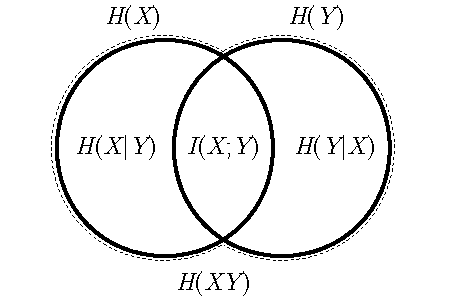
\includegraphics[width=6.5cm]{Venn1.pdf} \\[4ex]
\end{minipage}
\begin{minipage}[b]{6cm}
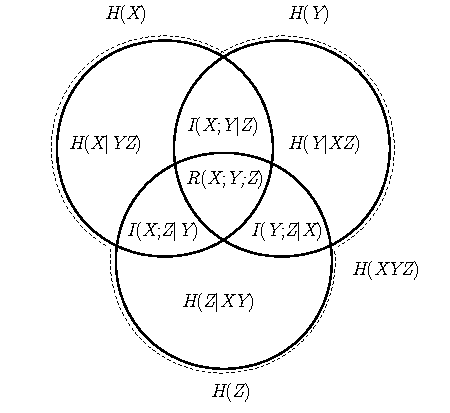
\includegraphics[width=8.5cm]{Venn2.pdf}
\end{minipage}
\else
\begin{minipage}[b]{6cm}
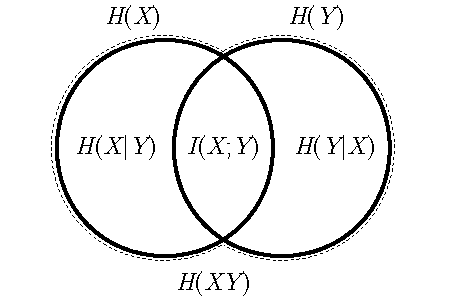
\includegraphics[width=6.5cm]{Venn1.eps} \\[4ex]
\end{minipage}
\begin{minipage}[b]{6cm}
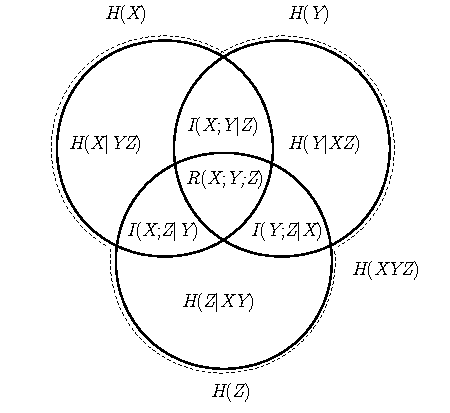
\includegraphics[width=8.5cm]{Venn2.eps}
\end{minipage}
\fi
%\end{center}
\vspace{-2ex}
\caption{Entropy diagram for two (left) and three (right) random variables. The areas encompassed by the dotted lines represent $H(XY)$ and $H(XYZ)$, respectively.}\label{fig:entropy-diagram}
\end{figure}

One subtlety with the entropy diagram for three random variables is that the ``area in the middle'', $R(X;Y;Z) = I(X;Y) - I(X;Y|Z)$, may be {\em negative}.



\section{Further Reading}
\begin{itemize}
\item Sections 2.1, 2.2, 3.1-3.3 of \CF
\item Sections 2.1, 2.2, 2.6 of \CT
\item For more background on probability theory, check for instance the \href{https://github.com/BasicProbability/LectureNotes/raw/master/fullscript/BasicProbabilityAndStatistics.pdf}{lecture
  script} of the Master of Logic course ``Basic Probability:Theory''
by Philip Schulz and Christian Schaffner.
\end{itemize}



%%% Local Variables:
%%% mode: latex
%%% TeX-master: "InfTheory3.tex"
%%% End:


\chapter{Source Coding}\label{ch:source-coding}
Suppose we sample $x$ from a distribution $P_X$ with image $\cal
X$. In the context of data compression, $P_X$ is typically called a
\term{source} that emits value $x \in {\cal X}$ with probability
$P_X(x)$. We want to compress (or encode) symbols $x$ sampled from
$P_X$ in such a way that we can later decompress (or decode) it reliably, without losing any information about the value $x$.

\begin{figure}[h]
\begin{center}
\begin{tikzpicture}
\draw[fill=black!5] (0,0) rectangle (2,2);
\node at (1,1.25) {$P_X$};
\node at (1,0.75) {(source)};

\draw[-latex] (2,1) -- (5,1);
\draw[fill=white,draw=none] (2.5,0) rectangle (4.5,2);
\node at (3.5,1.5) {$x$, with};
\node at (3.5,1) {probability};
\node at (3.5,0.5) {$P_X(x)$};

\draw[fill=black!5] (5,0) rectangle (7,2);
\node at (6,1.25) {encoding};
\node at (6,0.75) {function};

\draw[-latex] (7,1) -- (10,1);
\draw[fill=white,draw=none] (7.75,0) rectangle (9.25,2);
\node at (8.5,1.5) {compressed};
\node at (8.5,1) {version};
\node at (8.5,0.5) {of $x$};

\draw[fill=black!5] (10,0) rectangle (12,2);
\node at (11,1.25) {decoding};
\node at (11,0.75) {function};

\draw[-latex] (12,1) -- (13,1);
\node at (13.5,1) {$x$};
\end{tikzpicture}
\end{center}
\end{figure}

\noindent A counting argument shows that it is possible to encode the
elements of ${\cal X}$ by bit strings of length $n$, where $n=\lceil
\log (|{\cal X}|) \rceil $: we simply list all elements of ${\cal X}$,
and use the (binary) index of $x$ in the list as its encoding. 
Thus, to store or to transmit an element $x\in {\cal X}$, $n$ bits
of information always suffice. However, if not all $x \in \cal X$ are equally likely according to $P_X$, one should be able to
exploit this to achieve codes with shorter {\em average} length. The idea is to use encodings of varying lengths, assigning shorter codewords to the elements in ${\cal X}$ that have higher probabilities, and vice versa.
The question we answer in this chapter is: how short can such a code be (on average over repeated samples $x$ from $P_X$)?

We explore both \term{lossless} codes (where we want to recover the original data with certainty) and \term{lossy} codes (where with small probability, the data is lost).
%The average length of the code is inversely related the amount of information that is contained in $X$.


%Let $X$ be a random variable with image $\cal X$. A counting argument shows that it is possible to encode the elements of ${\cal X}$ by bit strings of length $n$, where $n=\lceil \log (|{\cal X}|) \rceil $: we simply list all elements of ${\cal X}$, and use the binary representation of their index in the list as the encoding. 
%Thus, to store or to transmit an element $x\in {\cal X}$, $n$ bits
%of information always suffice. However, if not all $x \in \cal X$ are equally likely with respect to $X$ (in this context typically called the \term{source}), one should be able to
%exploit this to achieve codes with shorter {\em expected} length. The idea is to use encodings of varying lengths, assigning shorter codewords to the elements in ${\cal X}$ that have higher probabilities, and vice versa.
%The question we answer in this chapter is: how short can such a code be (on average over the choice of~$x$)?




\section{Symbol Codes}
We start by investigating codes that encode a source one symbol at a time. Later on, we will also see codes that group the source symbols together into blocks.
\begin{definition}[Binary symbol code]
Let $P_X$ be the distribution of a random variable $X$ (with image ${\cal X}$). A binary symbol code for $P_X$ is an injective function $C : {\cal X} \to \strg$.

The \term{extended} code $C^* : {\cal X}^* \to \strg$ is defined by concatenation:
\[
C^*(x_1, ..., x_n) := C(x_1) | \cdots |C(x_n).
\]
Here, ${\cal X}^* = \bigcup_{n \in \N} {\cal X}^n \cup \set{\es}$, and $\es$ is the empty string.
\end{definition}
We often refer to the set of codewords, ${\cal C} = \im(C)$, as code and leave the actual encoding function $C$ implicit. 

The injectivity of $C$ ensures that we can always uniquely decode $C(x)$. However, if one transmits a sequence $x_1, \ldots, x_m\in {\cal X}$
(or stores them ``sequentially'') by sending the concatenation $C(x_1, ..., x_n)$, ambiguities may arise, namely in cases where it is possible to parse this long
string in two consistent but different ways. Indeed, injectivity of
the encoding function per se does not rule out that there exists a
positive integer $m'$ and elements $x'_1, \ldots, x'_{m'}\in {\cal X}$
such that $C(x_1)| \cdots | C(x_m)=C(x'_1)| \cdots | C(x'_{m'})$. Of course, this problem can be circumvented by introducing a special separation symbol. However, such a symbol might not be available, and maybe even more importantly, even if an additional symbol {\em is} available, then one can often create a better code by using it as an ordinary code symbol (in addition to 0 and 1) rather than as a special separation symbol. This is why it is interesting to study the following class of symbol codes:

\begin{definition}[Uniquely decodable code]
A binary symbol code $C : {\cal X} \to \strg$ is uniquely decodable if $C^*$ is injective as well.
\end{definition}

One convenient way to guarantee that a code is unique decodable is to require it to be prefix-free:
\begin{definition}[Prefix-free code]
A binary symbol code $C : {\cal X} \to \strg$ is prefix-free (or: \term{instantaneous}) if for all $x, x' \in \cal X$ with $x \neq x'$, $C(x)$ is {\em not} a prefix of $C(x')$.
\end{definition}

With a prefix-free encoding, the elements
$x_1, \ldots, x_m$ can be uniquely recovered from $C(x_1)|\cdots
|C(x_m)$, simply by reading the encoding from left to right one bit
at a time: by prefix-freeness it will remain unambiguous as reading
continues when the current word terminates and the next begins. This is a loose argument for the following:
\begin{proposition}\label{lemma:PF->UD}
If a code $\cal C$ is prefix-free and ${\cal C} \neq \set{\es}$ then $\cal C$ is uniquely decodable. 
\end{proposition}
The other direction does not hold: uniquely decodable codes need not be prefix-free. A prefix-free code is appealing from an efficiency point of view, as it allows to decode ``on the fly''. For a general uniquely decodable code one may possibly have to inspect all bits
in the entire string before being able to even recover the first word. 

\begin{example}\label{example:codes}
The following are three codes for the source $P_X$, with ${\cal X} = \{a,b,c,d\}$:
\[
\begin{array}{c | c | l | l | l | l}
x & P_X(x) & C_1(x) & C_2(x) & C_3(x) & C_4(x)\\
\hline
a & 1/2 & 00 & 0   & 0   & 0   \\
\hline
b & 1/4 & 01 & 10  & 010 & 01  \\
\hline
c & 1/8 & 10 & 110 & 01  & 011 \\
\hline
d & 1/8 & 11 & 111 & 10  & 111
\end{array}
\]
These codes can be visualised a as binary trees, with marked
codewords, as follows:
\begin{center}
%C1:
\begin{tikzpicture}
  [
    grow                    = right,
    sibling distance        = 2.5em,
    level distance          = 2.5em,
    edge from parent/.style = {draw},
    every node/.style       = {font=\footnotesize}
  ]
  \tikzstyle{level 1}=[sibling distance=5em]
  \tikzstyle{level 2}=[sibling distance=2.5em]
  \node [dummy] {}
    child { node [dummy] {}
      child { node [marked] {}
      	edge from parent node [below] {1} }
      child { node [marked] {} 
        edge from parent node [above] {0} }
      edge from parent node [below] {1} }
    child { node [dummy] {}
      child { node [marked] {}
      	edge from parent node [below] {1} }
      child { node [marked] {} 
        edge from parent node [above] {0} }
      edge from parent node [below] {1} };
\end{tikzpicture}
%
\qquad
%
%C2:
\begin{tikzpicture}
  [
    grow                    = right,
    sibling distance        = 2.5em,
    level distance          = 2.5em,
    edge from parent/.style = {draw},
    every node/.style       = {font=\footnotesize}
  ]
  \node [dummy] {}
    child { node [dummy] {}
      child { node [dummy] {}
        child { node [marked] {}
          edge from parent node [below] {1} }
        child { node [marked] {} 
          edge from parent node [above] {0} }
      	edge from parent node [below] {1} }
      child { node [marked] {} 
        edge from parent node [above] {0} }
      edge from parent node [below] {1} }
    child { node [marked] {}
      edge from parent node [above] {0} };
\end{tikzpicture}
%
\qquad
%
%C3:
\begin{tikzpicture}
  [
    grow                    = right,
    sibling distance        = 2.5em,
    level distance          = 2.5em,
    edge from parent/.style = {draw},
    every node/.style       = {font=\footnotesize}
  ]
  \tikzstyle{level 1}=[sibling distance=5em]
  \tikzstyle{level 2}=[sibling distance=2.5em]
  \node [dummy] {}
    child { node [dummy] {}
      child {node [dummy] {} 
        edge from parent node[below] {1} }
      child {node [marked] {}
        edge from parent node[above] {0} }
      edge from parent node [below] {1} }
    child { node [marked] {}
      child { node [marked] {}
        child { node [dummy] {}
          edge from parent node [below] {1} }
        child { node [marked] {} 
          edge from parent node [above] {0} }
      	edge from parent node [below] {1} }
      child { node [dummy] {} 
        edge from parent node [above] {0} }
      edge from parent node [above] {0} };
\end{tikzpicture}
%
\qquad
%
%C4:
\begin{tikzpicture}
  [
    grow                    = right,
    sibling distance        = 2.5em,
    level distance          = 2.5em,
    edge from parent/.style = {draw},
    every node/.style       = {font=\footnotesize}
  ]
  \tikzstyle{level 1}=[sibling distance=5em]
  \tikzstyle{level 2}=[sibling distance=2.5em]
  \node [dummy] {}
  	child { node [dummy] {} %1
  	  child { node [dummy] {} %11
  	    child { node [marked] {} %111
  	      edge from parent node [below] {1} }
  	    child { node [dummy] {} %110
  	      edge from parent node [above] {0} }
  	    edge from parent node [below] {1} }
  	  child { node [dummy] {} %10
  	    edge from parent node [above] {0} }
  	  edge from parent node [below] {1} }
  	child { node [marked] {} %0
  	  child { node [marked] {} %01
  	    child { node [marked] {} %011
  	      edge from parent node [below] {1} }
  	    child { node [dummy] {} %010
  	      edge from parent node [above] {0} }
  	    edge from parent node [below] {1} }
  	  child { node [dummy] {} %00
  	    edge from parent node [above] {0} }
  	  edge from parent node [above] {0} };
%  \node [dummy] {}
%    child { node [marked] {}
%      edge from parent node [below] {1} }
%    child { node [dummy] {}
%      child { node [marked] {}
%      	edge from parent node [below] {1} }
%      child { node [dummy] {} 
%        child { node [marked] {}
%          edge from parent node [below] {1} }
%        child { node [marked] {} 
%          edge from parent node [above] {0} }
%        edge from parent node [above] {0} }
%      edge from parent node [above] {0} };
\end{tikzpicture}
\\
$C_1$ {\hskip7em\relax} $C_2$ {\hskip8em\relax} $C_3$ {\hskip7em\relax} $C_4$ {\hskip6em\relax}
\end{center}
$C_1$ and $C_2$ are prefix-free, and therefore also uniquely
decodable. $C_3$ is not uniquely decodable, as $C_3(ad) = C_3(b)$.
$C_4$ is not prefix-free, but it is uniquely decodable, since it can
be decoded from right to left (it is ``postfix-free"). Note that the
binary trees for the prefix-free codes $C_1, C_2$ only have codewords at the leaves. (The same holds for the postfix-free code $C_4$).
\end{example}
For efficiency reasons, we are often interested in the average (expected) length of a code $C$:
\begin{definition}[Average length]
Let $\len(s)$ denote the length of a string $s \in \strg$. The (average) length of a code $C$ for a source $P_X$ is defined as
\[
\len_C(P_X) := \Exp[\len(C(X))] = \sum_{x \in \cal X} P_X(x) \len(C(x)) \, .
\]
\end{definition}
\begin{example} For the codes from Example~\ref{example:codes}, we
  obtain the following average codeword lengths: $\len_{C_1}(P_X) = 2,
  \len_{C_2}(P_X)=\len_{C_4}(P_X)=\frac{1}{2} \cdot 1 + \frac{1}{4} \cdot 2 +
  \frac{1}{8} \cdot 3 + \frac{1}{8} \cdot 3 = \frac{7}{4} = 1.75$ and
  $\len_{C_3}(P_X) =  \frac{1}{2} \cdot 1 + \frac{1}{4} \cdot 3 +
  \frac{1}{8} \cdot 2 + \frac{1}{8} \cdot 2 = \frac{7}{4} = 1.75 \,$. We see that the codes $C_2,C_3,C_4$ have a smaller average codeword length, but $C_2$ and $C_4$ are preferred over $C_3$ because their unique decodability. 

Notice that the individual codeword lengths of codes $C_2$ and $C_4$ correspond exactly to the surprisal values of $P_X$ in bits, e.g.\ $\ell(C_2(b)) = \ell(C_4(b))  = 2 = -\log P_X(b)$. Therefore, the computations of the entropy $H(X)$ and of the average code length $\ell_{C_2}(P_X)$ are exactly the same, and we have that $H(X) = \ell_{C_2}(P_X) = \ell_{C_4}(P_X)$. We will see in Section~\ref{sec:sourcecoding} below that this property characterizes optimal codes.
\end{example}

\begin{definition}[Minimal code length]
The minimal code length of a source $P_X$ is defined as
\[
\len_{\min}(P_X) := \min_{C \in \frak{C}} \len_C(P_X)
\]
where $\frak{C}$ is some class of codes, for example the set of all prefix-free codes (resulting in $\len_{\min}^{\text{\rm p.f.}}$), or the set of all uniquely decodable codes (resulting in $\len_{\min}^{\text{\rm u.d.}}$). 
\end{definition}



\section{Kraft's Inequality}\label{sec:kraft}
As argued, prefix-freeness is a nice feature, but it is also considerably more restrictive than mere unique decodability; thus, it is natural to ask: how much do we lose (in terms of the average codeword length) by requiring the encoding to be prefix-free rather than merely uniquely decodable? Surprisingly, the answer is: {\em nothing}. In this section, we will show that the length of an optimal prefix-free code and the length of an optimal uniquely decodable code coincide. In the next section, we will see that these lengths are essentially given by the Shannon entropy.

\begin{theorem}[Kraft's inequality]
There exists a prefix-free code with image ${\cal C} = \set{c_1, ..., c_m}$ and codeword lengths $\len_i := \len(c_i)$, if and only if
\[
\sum_{i=1}^m 2^{-\ell_i} \leq 1.
\]
\end{theorem}
\begin{proof}
For the forward direction, suppose we have a prefix-free code $C$ with image ${\cal C} = \set{c_1, ..., c_m}$ and codeword lengths $\len_i := \len(c_i)$. View this code as a tree, with codewords only on the leaves (but not necessarily all the leaves), and assign a weight of $2^{-d}$ to every node in the tree at depth $d$ (including the leaves):
%\begin{figure}[h]
\begin{center}
\begin{tikzpicture}
  [
    grow                    = right,
    sibling distance        = 2.5em,
    level distance          = 2.5em,
    edge from parent/.style = {draw},
    every node/.style       = {font=\footnotesize}
  ]
  
  \draw[dashed] (0,-2) -- (0,2);
  \draw[dashed] (2.5em,-2) -- (2.5em,2);
  \draw[dashed] (5em,-2) -- (5em,2);
  \draw[dashed] (7.5em,-2) -- (7.5em,2);
  \tikzstyle{level 1}=[sibling distance=5em]
  \tikzstyle{level 2}=[sibling distance=2.5em]
  \node [dummy] {}
    child { node [dummy] {}
      child {node [marked] {} 
        edge from parent node[below] {1} }
      child {node [dummy] {}
        child { node [marked] {}
          edge from parent node [below] {1} }
        child { node [marked] {} 
          edge from parent node [above] {0} }
        edge from parent node[above] {0} }
      edge from parent node [below] {1} }
    child { node [dummy] {}
      child { node [dummy] {}
      	edge from parent node [below] {1} }
      child { node [marked] {} 
        edge from parent node [above] {0} }
      edge from parent node [above] {0} };
  \node[anchor=south] at (0    ,2) {$2^0$};
  \node[anchor=south] at (2.5em,2) {$2^{-1}$};
  \node[anchor=south] at (5em  ,2) {$2^{-2}$};
  \node[anchor=south] at (7.5em,2) {$2^{-3}$};
\end{tikzpicture}
\end{center}
%\end{figure}

\noindent Note that the weight of each node is exactly the sum of the weight of its direct children, and thereby that the weight of the root is exactly the weight of all of the leaves. Since every codeword $c_i$ resides on a leaf of depth $\ell_i$ (but not all leaves are necessarily occupied), the weight of the root is \emph{at least} the sum of all the codeword weights:
\begin{align}
\sum_{i=1}^{m} 2^{-\ell_i} \leq 2^0 = 1.
\end{align}

For the backward direction, we build a code ${\cal C} = \{c_1, ..., c_m\}$ with $\ell(c_i) = \len_i$ by selecting the appropriate leaves of a binary tree as codewords, assigning the most `expensive' (i.e.\ those with small depth) first. We proceed by induction on the number of codewords, $m$:

For $m = 1$, the construction is clear: we can assign any string of length $\len_1$ to represent the single codeword.

For $m > 1$, assume without loss of generality that $\ell_1 \leq \cdots \leq \ell_{m-1} \leq \ell_{m}$. We will first try to build a code with $(m-1)$ code words, of lengths $\ell_1, ..., \ell_{m-2}, (\ell_{m-1} - 1)$. In order to be able to invoke the induction hypothesis, we do need to check that
\begin{align}
\left(\sum_{i=1}^{m-2} 2^{-\ell_{i}}\right) + 2^{-(\ell_{m-1} - 1)} \leq 1.
\end{align}
This can be seen by first noting that
\begin{align}
1 \ > \ 1 - 2^{-\len_m} \ \geq \ \sum_{i=1}^{m-1} 2^{-\len_i} \ = \ \sum_{i=1}^m \frac{2^{\len_{m-1} - \len_i}}{2^{\len_{m-1}}} \ = \ \frac{\sum_{i=1}^{m-1} 2^{\len_{m-1} - \len_i}}{2^{\len_{m-1}}}.
\end{align}
Thus, on the right-hand side, we end up with a fraction of the form $\frac{a}{b} < 1$, where $a$ and $b$ are both integers, with $a < b$. In this case it must follow that $a + 1 \leq b$, and hence $\frac{a+1}{b} \leq 1$. So we get
\begin{align}
1
\ \geq \ \frac{\left(\sum_{i=1}^{m-1} 2^{\len_{m-1} - \len_i}\right) + 1}{2^{\len_{m-1}}}
&= \ \left(\sum_{i=1}^{m-1} 2^{-\len_i}\right) + 2^{-\len_{m-1}}\nonumber\\
&= \ \left(\sum_{i=1}^{m-2} 2^{-\len_i}\right) + 2\cdot 2^{-\len_{m-1}}\nonumber\\
&= \ \left(\sum_{i=1}^{m-2} 2^{-\ell_{i}}\right) + 2^{-(\ell_{m-1} - 1)},
\end{align}
as desired. So we invoke the induction hypothesis to create a prefix-free code ${\cal C}' = \{c'_1, ..., c'_{m-1}\}$ with lengths $\len_1, ..., \len_{m-2}, (\len_{m-1} - 1)$. The new code ${\cal C}$ is then constructed by setting $c_i = c'_i$ for all $i \leq m-2$, and furthermore setting $c_{m-1} = c'_{m-1}|0$ and $c_m = c'_{m-1}|10\cdots 0$, padding with enough zeroes to achieve $\len(c_m) = \len_m$. This new code is necessarily also prefix-free.

The following image illustrates the induction step for $\ell_1 = \ell_2 = \ell_3 = 2$ and $\ell_4 = 3$. The code is constructed from a prefix-free code ${\cal C}'$ with code lengths $2, 2$ and 1 by replacing the bottom codeword (of length 1) with two new codewords (of lengths 2 and 3).

%\begin{figure}[h]
\begin{center}
\begin{tikzpicture}
  [
    grow                    = right,
    sibling distance        = 2.5em,
    level distance          = 2.5em,
    edge from parent/.style = {draw},
    every node/.style       = {font=\footnotesize}
  ]
  \tikzstyle{level 1}=[sibling distance=5em]
  \tikzstyle{level 2}=[sibling distance=2.5em]
  \node [dummy] {}
    child { node [marked] {}
      edge from parent node [below] {1} }
    child { node [dummy] {}
      child { node [marked] {}
      	edge from parent node [below] {1} }
      child { node [marked] {} 
        edge from parent node [above] {0} }
      edge from parent node [above] {0} };
  
  \node[anchor=north] at (2.5em,-2.25) {${\cal C}' = \set{00, 01, 1}$};
\end{tikzpicture}
\qquad
\begin{tikzpicture}
\node at (0,0) {$\Rightarrow$};
\end{tikzpicture}\qquad
\begin{tikzpicture}
  [
    grow                    = right,
    sibling distance        = 2.5em,
    level distance          = 2.5em,
    edge from parent/.style = {draw},
    every node/.style       = {font=\footnotesize}
  ]
  \tikzstyle{level 1}=[sibling distance=5em]
  \tikzstyle{level 2}=[sibling distance=2.5em]
  \node [dummy] {}
    child { node [dummy] {}
      child {node [dummy] {} 
        child { node [dummy] {}
          edge from parent node [below] {1} }
        child { node [marked] {} 
          edge from parent node [above] {0} }
        edge from parent node[below] {1} }
      child {node [marked] {}
        edge from parent node[above] {0} }
      edge from parent node [below] {1} }
    child { node [dummy] {}
      child { node [marked] {}
      	edge from parent node [below] {1} }
      child { node [marked] {} 
        edge from parent node [above] {0} }
      edge from parent node [above] {0} };
  \node[anchor=north] at (3.75em,-2.25) {${\cal C} = \set{00, 01, 10, 110}$};
\end{tikzpicture}
\end{center}
%\end{figure}
\end{proof}
A stronger version of Kraft's inequality holds as well, this time for uniquely decodable codes:
\begin{theorem}[McMillan inequality]
For a uniquely decodable code with image ${\cal C} = \set{c_1, ..., c_m}$ and codeword lengths $\len_i := \len(c_i)$, it holds that
\[
\sum_{i=1}^m 2^{-\ell_i} \leq 1.
\]
\end{theorem}
\begin{proof}
Let ${\cal C}$ be a uniquely decodable code as in the theorem statement. We can write
\begin{align}
S := \sum_{c \in \cal C} \frac{1}{2^{\len(c)}} = \sum_{\ell = L_{\min}}^{L_{\max}} \frac{n_\ell}{2^\ell} 
\end{align}
where $L_{\min} = \min_{c \in \cal C} \len(c)$, $L_{\max} = \max_{c \in \cal C} \len(c)$, and $n_{\ell} = |\Set{c \in {\cal C}}{\len(c) = \ell}|$. Furthermore, for any $k \in \N$,  consider the $k$th power of $S$,
\begin{align}
S^k = \sum_{c_1,\ldots,c_k \in \mathcal{C}^k} \frac{1}{2^{\len(c_1)+\ldots+\len(c_k)}} = \sum_{\ell = k L_{\min}}^{k L_{\max}} \frac{n_\ell^{(k)}}{2^\ell} 
\end{align}
where $n_\ell^{(k)}$ is defined as $n_\ell^{(k)} = \big|\SET[\big]{(c_1,\ldots,c_k) \in {\cal C}^k}{\sum_i\len(c_i) = \len(c_1|\ldots|c_k) = \ell}\big|$. Note that
\begin{align}
n_\ell^{(k)} = \sum_{x \in \set{0,1}^{\ell}} \big|\SET{(c_1,\ldots,c_k) \in {\cal C}^k}{\,c_1|\ldots|c_k = x}\big| \leq \sum_{x \in \set{0,1}^{\ell}} 1 = 2^{\ell}
\end{align}
where the inequality follows from the unique decodability of $\cal C$. Thus, we can conclude that 
\begin{align}
S^k \leq (L_{\max} - L_{\min}) \cdot k 
\end{align}
for all $k \in \N$, so $S^k$ grows at most linearly in $k$, from which follows that $S \leq 1$ (for if not, $S^k$ would grow exponentially in $k$).
\end{proof}
Kraft's and McMillan's inequality together lead to the conclusion that the lengths of an optimal prefix-free code and an optimal uniquely decodable code coincide:
\begin{corollary}
Let $P_X$ be a source. For every uniquely decodable code $C$, there exists a prefix-free code $C'$ such that $\ell_C(P_X) = \ell_{C'}(P_X)$. Hence,
\[
\ell_{\min}^{\text{\rm p.f.}}(P_X) = \ell_{\min}^{\text{\rm u.d.}}(P_X).
\]
\end{corollary}
From now on, we will just write $\len_{\min}(P_X)$ to denote either of these measures for average length. A code $C$ for which $\len_C(P_X) = \len_{\min}(P_X)$ is called \term{optimal} for the source $P_X$. 




\section{Shannon's Source-Coding Theorem} \label{sec:sourcecoding}
We now know that prefix-free codes can achieve the same minimal code lengths for a source $P_X$ as the more general class of uniquely decodable codes. How small is this minimal code length in general? In this section we explore the following relation between the minimal code length and the entropy of the source:
\begin{theorem}[Shannon's source-coding theorem (for symbol codes)]
For any source $P_X$, we have the following bounds:
\[
H(X) \leq \len_{\min}(P_X) \leq H(X) + 1.
\]
\end{theorem}
\begin{proof}
The proof relies on Kraft's inequality (Section~\ref{sec:kraft}). Let $C$ be a code, and write $\len_x$ for $\len(C(x))$ as a notational convenience. For the lower bound, we have that
\begin{align}
H(X) - \len_C(P_X) &= - \sum_{x \in {\cal X}} P_X(x) \log(P_X(x)) - \sum_{x \in X} P_X(x) \len_x\nonumber\\
&=  \sum_{x \in {\cal X}} P_X(x) \left(-\log(P_X(x)) - \log\left(2^{\len_x}\right)\right)\nonumber\\
&=  \sum_{x \in {\cal X}} P_X(x) \log \left(\frac{1}{P_X(x)\cdot 2^{\len_x}}\right)\nonumber\\
&\leq \log\left(\sum_{x \in {\cal X}} \frac{1}{2^{\len_x}}\right) &&\mbox{(by Jensen's inequality)}\nonumber\\
&\leq \log(1) = 0&&\mbox{(by Kraft's inequality)}
\end{align}
For the upper bound, let us denote by $\len_x$ the surprisal value in bits rounded up to the next integer, i.e.\ for any $x \in {\cal X}$,
\begin{align}
\len_x := \left\lceil\log\frac{1}{P_X(x)}\right\rceil,
\end{align}
and note that
\begin{align}
\sum_{x \in {\cal X}} 2^{-\len_x} \leq \sum_{x \in {\cal X}} 2^{-\log\frac{1}{P_X(x)}} = \sum_{x \in {\cal X}} P_X(x) = 1.
\end{align}
Therefore, by Kraft's inequality, there exists a prefix-free code $C$ such that $\len(C(x)) = \len_x$ for all $x \in {\cal X}$. This code satisfies
\begin{align}
\len_C(P_X) &= \sum_{x \in {\cal X}} P_X(x) \len_x \nonumber\\
&\leq \sum_{x \in {\cal X}} P_X(x) \left(\log \frac{1}{P_X(x)} + 1 \right)\nonumber\\
&= -\sum_{x \in {\cal X}} P_X(x)\log P_X(x) + \sum_{x \in {\cal X}} P_X(x) \nonumber\\
&= H(X) + 1.
\end{align}
We have thus constructed a code $C$ with $\len_C(P_X) \leq H(X) + 1$, so $\len_{\min}(P_X) \leq H(X) + 1$.
\end{proof}

\section{Huffman Codes}
Shannon's source-coding theorem shows us that in theory, the minimal code length for a source $P_X$ is roughly $H(X)$. In this section we will investigate \term{Huffman codes}, which provide an explicit and neat construction for optimal prefix-free codes. A binary Huffman code for a source $P_X$ is constructed by iteratively pairing the two symbols with the smallest probability together, building a binary tree on the way. This is best explained by example:

\begin{example}[Binary Huffman code]\label{example:bin-huffman}
Let the random variable $X$ be given with $\mathcal{X} = \{a,b,c,d,e\}$ and $P_X(a) = P_X(b) = 0.25$, $P_X(c) = 0.2$, and $P_X(d) = P_X(e) = 0.15$. The following is a binary Huffman code for $P_X$:
\begin{center}
\begin{tikzpicture}
\pgfmathsetmacro{\dist}{0.75}
\node at (0,5*\dist) {$x$};
\node at (0,4*\dist) {$a$};
\node at (0,3*\dist) {$b$};
\node at (0,2*\dist) {$c$};
\node at (0,1*\dist) {$d$};
\node at (0,0*\dist) {$e$};
\draw (-0.5,4.5*\dist) -- (1.5,4.5*\dist);
\draw (0.5,-0.5*\dist) -- (0.5,5.5*\dist);
\node at (1,5*\dist) {$P_X(x)$};
\node at (1,4*\dist) {$0.25$};
\node at (1,3*\dist) {$0.25$};
\node at (1,2*\dist) {$0.2$};
\node at (1,1*\dist) {$0.15$};
\node at (1,0*\dist) {$0.15$};

%STEP 1
\node at (2,0*\dist) {\small $1$};
\node at (2,1*\dist) {\small $0$};
\draw (1.5,0*\dist) -- (2.5,0.5*\dist);
\draw (1.5,1*\dist) -- (2.5,0.5*\dist);
\node[anchor=west] at (2.5,0.5*\dist) {$0.3$};
%\node[anchor=west] at (2.5,2*\dist) {$0.2$};
%\node[anchor=west] at (2.5,3*\dist) {$0.25$};
%\node[anchor=west] at (2.5,4*\dist) {$0.25$};

%STEP 2
\node at (4,2*\dist) {\small $1$};
\node at (4,3*\dist) {\small $0$};
\draw[dotted] (1.5,2*\dist) -- (3.5,2*\dist);
\draw[dotted] (1.5,3*\dist) -- (3.5,3*\dist);
\draw (3.5,2*\dist) -- (4.5,2.5*\dist);
\draw (3.5,3*\dist) -- (4.5,2.5*\dist);
\node[anchor=west] at (4.5,2.5*\dist) {$0.45$};
%\node[anchor=west] at (4.5,0.5*\dist) {$0.3$};
%\node[anchor=west] at (4.5,4*\dist) {$0.25$};

%STEP 3
\node at (6,0.5*\dist) {$1$};
\node at (6,3*\dist) {$0$};
\draw[dotted] (3.2,0.5*\dist) -- (5.5,0.5*\dist);
\draw[dotted] (1.5,4*\dist) -- (5.5,4*\dist);
\draw (5.5,0.5*\dist) -- (6.5,1*\dist);
\draw (5.5,4*\dist) -- (6.5,1*\dist);
%\node[anchor=west] at (6.5,2.5*\dist) {$0.45$};
\node[anchor=west] at (6.5,1*\dist) {$0.55$};

%STEP 4
\node at (8,1.25*\dist) {$1$};
\node at (8,2.5*\dist) {$0$};
\draw[dotted] (5.3,2.5*\dist) -- (7.5,2.5*\dist);
\draw (7.5,2.5*\dist) -- (8.5,2*\dist);
\draw (7.5,1*\dist) -- (8.5,2*\dist);
\node[anchor=west] at (8.5,2*\dist) {$1$};

%RESULT
\node at (10,5*\dist) {code};
\draw (9.5,4.5*\dist) -- (10.5,4.5*\dist);
\node at (10,4*\dist) {$10$};
\node at (10,3*\dist) {$00$};
\node at (10,2*\dist) {$01$};
\node at (10,1*\dist) {$110$};
\node at (10,0*\dist) {$111$};
\end{tikzpicture}
\end{center}
We build up the tree from left to right, pairing the symbols (or groups of symbols) with smallest (combined) probabilities at every step. The codeword for every symbol is then determined by following the branches of the tree \emph{from right to left} until the symbol is reached. Note that this way, the symbols with the smallest probabilities get assigned the longest codewords (paths).

The average codeword length for this code is
\begin{align}
0.25 \cdot 2 + 0.25 \cdot 2 + 0.2 \cdot 2 + 0.15 \cdot 3 + 0.15 \cdot 3 = 2.3. 
\end{align}
This very close to the entropy $H(X) \approx 2.285$. The average codeword length lies between $H(X)$ and $H(X) + 1$.
\end{example}

The above was an example of how to construct \emph{binary} Huffman codes. We can also generate Huffman codes for larger alphabets, resulting in ternary, quaternary, or, more generally, \term{$d$-ary Huffman codes}.

\begin{example}[Ternary Huffman code]\label{example:ter-huffman}
We build a Huffman code with the alphabet $\set{0,1,2}$ for the same distribution as in Example~\ref{example:bin-huffman}.
\begin{center}
\begin{tikzpicture}
\pgfmathsetmacro{\dist}{0.75}
\node at (0,5*\dist) {$x$};
\node at (0,4*\dist) {$a$};
\node at (0,3*\dist) {$b$};
\node at (0,2*\dist) {$c$};
\node at (0,1*\dist) {$d$};
\node at (0,0*\dist) {$e$};
\draw (-0.5,4.5*\dist) -- (1.5,4.5*\dist);
\draw (0.5,-0.5*\dist) -- (0.5,5.5*\dist);
\node at (1,5*\dist) {$P_X(x)$};
\node at (1,4*\dist) {$0.25$};
\node at (1,3*\dist) {$0.25$};
\node at (1,2*\dist) {$0.2$};
\node at (1,1*\dist) {$0.15$};
\node at (1,0*\dist) {$0.15$};

%STEP 1
\node at (2,0*\dist) {\small $2$};
\node at (1.75,1.25*\dist) {\small $1$};
\node at (2,2*\dist) {\small $0$};
\draw (1.5,0*\dist) -- (2.5,1*\dist);
\draw (1.5,1*\dist) -- (2.5,1*\dist);
\draw (1.5,2*\dist) -- (2.5,1*\dist);
\node[anchor=west] at (2.5,1*\dist) {$0.5$};

%STEP 2
\node at (4.25,1.75*\dist) {\small $2$};
\node at (3.75,3.25*\dist) {\small $1$};
\node at (4,4*\dist) {\small $0$};
\draw (3.5,1*\dist) -- (4.5,3*\dist);
\draw (3.5,3*\dist) -- (4.5,3*\dist);
\draw (3.5,4*\dist) -- (4.5,3*\dist);
\draw[dotted] (1.5,3*\dist) -- (3.5,3*\dist);
\draw[dotted] (1.5,4*\dist) -- (3.5,4*\dist);
\node[anchor=west] at (4.5,3*\dist) {$1$};

%RESULT
\node at (6,5*\dist) {code};
\draw (5.5,4.5*\dist) -- (6.5,4.5*\dist);
\node at (6,4*\dist) {$0$};
\node at (6,3*\dist) {$1$};
\node at (6,2*\dist) {$20$};
\node at (6,1*\dist) {$21$};
\node at (6,0*\dist) {$22$};
\end{tikzpicture}
\end{center}
\end{example}

\begin{exercise}\label{exercise:ter-huffman}
Use the above procedure to construct a ternary code for the source $P_X$ with $\mathcal{X} = \set{a,b,c,d,e,f}$ and $P_X(a) = P_X(b) = 0.25$, $P_X(c) = 0.2$, $P_X(d) = P_X(e) = P_X(f) = 0.1$. Can you find another code with a smaller average codeword length?
\end{exercise}
We have to be careful, because with an alphabet size of greater than 2, the above procedure does not always give an optimal code! In fact, a $d$-ary code is only optimal if $|\mathcal{X}|$ is of the form $k(d-1)+1$ for some $k \in \mathbb{N}$. This ensures that at every step, we can combine exactly $d$ symbols to use the alphabet at full capacity. The ternary code in Example~\ref{example:ter-huffman} is optimal because $|\mathcal{X}| = 5 = 2(3-1) + 1$, but the code you constructed in Exercise~\ref{exercise:ter-huffman} is not. To remedy this, one can add one or more `dummy' symbols to the source (each with probability zero) until an appropriate size of $\mathcal{X}$ of the form $|\mathcal{X}| = k(d-1)+1$ for some $k \in \mathbb{N}$ is reached. The codewords for those dummy symbols are discarded at the end.

It turns out that Huffman codes indeed have optimal code length (see \CT, Section 5.8).

\begin{theorem}[Optimality of Huffman codes]
Let $P_X$ be a source, and let $C^*$ be the associated Huffman code. For any other uniquely decodable code $C'$ with the same alphabet,
\[
\len_{C^*}(P_X) \leq \len_{C'}(P_X).
\]
\end{theorem}
% todo: add proof?

\begin{example}[20 questions]
In the game of `20 questions' (20Q) the goal is to identify an object from a set of objects using (at most) 20 yes/no questions. Please go and \href{http://www.20q.net/}{play it online} right now if you have never heard of it before.  Assume we know the probability distribution $P_X$ over all possible objects, what is the most efficient sequence of questions to ask in order to determine the object? We can use Huffman coding to answer this question!

On the one hand, the Huffman code for $P_X$ has optimal average code length and we could (in principle) ask the player about the first, second, third, etc.\ bit of the object in question (admittedly, these questions would be rather boring...). On the other hand, we can see the sequence of (questions and) answers as the `code' for an object, because every object as a unique sequence of yes/no answers. The number of questions asked is the length of the codeword. By Shannon's source-coding theorem,
\[
H(X) \leq \mbox{expected number of questions} \leq H(X) + 1,
\]
and the Huffman code procedure can be used to determine the optimal sequence of questions.
\end{example}
As we have seen, the average codeword length of Huffman codes is theoretically optimal. However, Huffman codes (and symbol codes in general) still have a number of disadvantages:
\begin{itemize}
\item When compressing, for example, an English text symbol-by-symbol, the probability distribution for each position may depend on the string of text that precedes it: for example, the letter \texttt{n} is a lot more likely than the letter \texttt{a} if it comes after the string \texttt{informatio}. Given this change of distribution, the Huffman code may not produce the shortest possible code. This can be resolved by recomputing the Huffman code after every symbol, but this results in a lot of overhead.
\item The average codeword length is upper bounded by $H(X) + 1$. This additive cost of 1 bit is fine when $H(X)$ is very large, but can be a significant overhead when $H(X)$ is small itself.
\end{itemize}

\section{Arithmetic Codes}
In this section, we study a different kind of code that can handle context-dependent distributions, unlike the Huffman code.

\begin{definition}[Standard binary representation]
The standard binary representation of a real number $r \in [0,1)$ is a (possibly infinite) string of bits $c_1c_2\cdots$ such that
\[
r = \sum_i c_i \cdot 2^{-i},
\]
where by convention, 0 is represented by the string 0.
\end{definition}
Not all reals in $[0,1)$ have a finite representation, but any interval $[a,b)$ with $0 \leq a < b \leq 1$ contains at least one number with a finite binary representation.
\begin{example}
The following table lists some numbers $r \in [0,1)$ and their standard binary representation.

\[
\begin{array}{c | c}
r & \mbox{binary representation of } r\\\hline
1/2 & 1\\
1/3 & 01010101\cdots\\
1/4 & 01\\
3/4 & 11\\
13/16 & 1101\\
13/32 & 01101\\
\end{array}
\]
Note that 1101 is also the binary form of the natural number 13. Adding a 0 on the left divides the represented value by 2.
\end{example}
These binary representations of numbers in the interval $[0,1)$ give rise to a very elegant code: 
\begin{definition}[Arithmetic code]\label{def:arithmetic}
Given a source $P_X$ with $\mathcal{X} = \{x_1, .., x_m\}$, construct the arithmetic code as follows. Divide the interval $[0,1)$ into disjoint subintervals $I_{x_j} = [a_j, a_{j+1})$, where $a_1, ..., a_{m+1}$ are defined such that $a_{j+1} - a_j = P_X(x_j)$, and $a_1 = 0, a_{m+1} = 1$.

The encoding $AC(x_j)$ of the element $x_j$ is the (shortest possible) standard binary representation of some number in the interval $I_{x_j}$. 
\end{definition}

\begin{example}\label{example:arithmetic}
Let $X$ be a random variable with $\mathcal{X} = \set{1,2,3}$ and $P_X(1) = \frac{1}{2}$, $P_X(2) = P_X(3) = \frac{1}{4}$. The arithmetic code is constructed by first determining the intervals:
\begin{center}
\begin{tikzpicture}
\draw (0,0) -- (5,0);
\draw node at (0,0) {$[$};
\draw node at (2.5,0) {$[$};
\draw node at (3.75,0) {$[$};
\draw node at (2.45,0) {$)$};
\draw node at (3.7,0) {$)$};
\draw node at (4.95,0) {$)$};
\draw[anchor=north] node at (0,-0.2) {$0$};
\draw[anchor=north] node at (2.5,-0.2) {$1/2$};
\draw[anchor=north] node at (3.75,-0.2) {$3/4$};
\draw[anchor=north] node at (5,-0.2) {$1$};
%
\draw[-latex] (0,1) -- (0,0.4);
\draw[-latex] (2.5,1) -- (2.5,0.4);
\draw[-latex] (3.75,1) -- (3.75,0.4);
\draw[anchor=south] node at (0,1) {$\mathcal{C}(1)$};
\draw[anchor=south] node at (2.5,1) {$\mathcal{C}(2)$};
\draw[anchor=south] node at (3.75,1) {$\mathcal{C}(3)$};
\end{tikzpicture}
\end{center}
This image results in the arithmetic code $\mathcal{C}$ with $\mathcal{C}(1) = 0$ (the representation of 0), $\mathcal{C}(2) = 1$ (the representation of $\frac{1}{2}$), $\mathcal{C}(2) = 11$ (the representation of $\frac{3}{4}$).

For $P_X$, the codewords happen to fall exactly \emph{on} the boundaries of the intervals. This is not always the case, however. The same code would have resulted from this procedure if we started with the random variable $Y$ with $\mathcal{Y} = \set{1,2,3}$ and $P_Y(1) = P_Y(2) = 0.3$ and $P_Y(3) = 0.4$:

\begin{center}
\begin{tikzpicture}
\draw (0,0) -- (5,0);
\draw node at (0,0) {$[$};
\draw node at (1.5,0) {$[$};
\draw node at (3,0) {$[$};
\draw node at (1.45,0) {$)$};
\draw node at (2.95,0) {$)$};
\draw node at (4.95,0) {$)$};
\draw[anchor=north] node at (0,-0.2) {$0$};
\draw[anchor=north] node at (2.5,-0.2) {$0.3$};
\draw[anchor=north] node at (3.75,-0.2) {$0.6$};
\draw[anchor=north] node at (5,-0.2) {$1$};
%
\draw[-latex] (0,1) -- (0,0.4);
\draw[-latex] (2.5,1) -- (2.5,0.4);
\draw[-latex] (3.75,1) -- (3.75,0.4);
\draw[anchor=south] node at (0,1) {$\mathcal{C}(1)$};
\draw[anchor=south] node at (2.5,1) {$\mathcal{C}(2)$};
\draw[anchor=south] node at (3.75,1) {$\mathcal{C}(3)$};
\end{tikzpicture}
\end{center}

\end{example}


\begin{proposition}\label{prop:arithmetic-length}
For any $(X,P_X)$, the arithmetic code has average length $\len_{AC}(P_X) \leq H(X) + 1$.
\end{proposition}
\begin{proof}
Let $x \in \mathcal{X}$, and define $\len_x := \lceil \log (1/P_X(x))\rceil$ to be the rounded surprisal value of $x$. Then
\begin{align}
2^{-\len_x} = 2^{-\lceil \log (1/P_X(x))\rceil} \leq 2^{-\log (1/P_X(x))} = 2^{\log P_X(x)} = P_X(x).
\end{align}
Therefore, since the size of the interval $I_x$ is $P_X(x)$, there must exist $0 \leq s_x < 2^{\len_x}$ such that $s_x \cdot 2^{-\len_x}$ lies in the interval $I_x$. This number $s_x \cdot 2^{-\len_x}$ has a binary representation of length $\len_x \leq -\log P_X(x) + 1$. Repeating this argument for every $x$, we obtain
\begin{align}
\len_{AC}(P_X) = \mathbb{E}[\len(AC(X))] = \sum_x P_X(x) \len(AC(x)) \leq \sum_x P_X(x) (-\log P_X(x) + 1) = H(X) + 1.
\end{align}
\end{proof}

As we can see from Example~\ref{example:arithmetic}, this construction for arithmetic codes does not necessarily yield prefix-free codes. However, at the expense of one extra bit of code (on average), the construction can be adapted into a prefix-free code. One example of this is the \term{Shannon-Fano-Elias code} (see \CT, Section 5.9 or \href{https://en.wikipedia.org/wiki/Shannon%E2%80%93Fano%E2%80%93Elias_coding}{Wikipedia}), which provides a more sophisticated way of selecting a number within each interval than simply selecting the number with the shortest binary representation. This alternative selection procedure ensures prefix-freeness. Another option is to select \emph{binary intervals} within each interval:

\begin{definition}[Binary interval]
A binary interval is an interval of the form
\[
\left[\frac{s}{2^{\len}}, \frac{s+1}{2^{\len}}\right)
\]
with $s, \len \in \mathbb{N}$ and $0 \leq s < 2^{\len}$. The \term{name} of the interval is the binary representation of $s$ (as a natural number) padded with zeroes on the left to reach length $\len$.
\end{definition}

\begin{definition}[Arithmetic code (prefix-free version)]
The prefix-free arithmetic code is identical to Definition~\ref{def:arithmetic}, except that the encoding $AC^{pf}(x_j)$ of the element $x_j$ is now the name of the largest binary interval that fits entirely in $I_{x_j}$.
\end{definition}
Similarly to Proposition~\ref{prop:arithmetic-length}, it can be shown that for any source  $P_X$, $\len_{AC^{pf}}(P_X) \leq H(X) + 2$. Note that we get prefix-freeness only at the expense of an extra bit on average.

\begin{example}
Let $Y$ be the random variable as in Example~\ref{example:arithmetic}, that is, $P_Y(1) = P_Y(2) = 0.3$ and $P_Y(3) = 0.4$. The prefix-free code for $Y$ is constructed as follows:

\begin{center}
\begin{tikzpicture}
\filldraw[draw=none,fill=ocre,opacity=0.5] (0,-0.25) rectangle (1.25,0.25);
\filldraw[draw=none,fill=ocre,opacity=0.5] (1.875,-0.25) rectangle (2.5,0.25);
\filldraw[draw=none,fill=ocre,opacity=0.5] (3.75,-0.25) rectangle (5,0.25);
%
\draw (0,0) -- (5,0);
\draw node at (0,0) {$[$};
\draw node at (1.5,0) {$[$};
\draw node at (3,0) {$[$};
\draw node at (1.45,0) {$)$};
\draw node at (2.95,0) {$)$};
\draw node at (4.95,0) {$)$};
\draw[anchor=north] node at (0,-0.2) {$0$};
\draw[anchor=north] node at (2.5,-0.2) {$0.3$};
\draw[anchor=north] node at (3.75,-0.2) {$0.6$};
\draw[anchor=north] node at (5,-0.2) {$1$};
%
\draw[dotted] (0,0) -- (0,0.5);
\draw[dotted] (1.25,0) -- (1.25,0.5);
\draw[dotted] (1.875,0) -- (1.875,0.5);
\draw[dotted] (2.5,0) -- (2.5,0.5);
\draw[dotted] (3.75,0) -- (3.75,0.5);
\draw[dotted] (5,0) -- (5,0.5);
\draw[anchor=south] node at (0,0.5)     {$\frac{0}{4}$};
\draw[anchor=south] node at (1.25,0.5)  {$\frac{1}{4}$};
\draw[anchor=south] node at (1.875,0.5) {$\frac{3}{8}$};
\draw[anchor=south] node at (2.5,0.5)   {$\frac{4}{8}$};
\draw[anchor=south] node at (3.75,0.5)  {$\frac{3}{4}$};
\draw[anchor=south] node at (5,0.5)     {$\frac{4}{4}$};
\end{tikzpicture}
\end{center}
This results in the codewords $\mathcal{C}(1) = 00$, $\mathcal{C}(2) = 011$, and $\mathcal{C}(3) = 11$.
\end{example}
The arithmetic code is slightly less efficient than the Huffman code in terms of average codeword length. A big advantage is the way it is able to adapt to changing distributions, such as when we are encoding a stream of English text. Suppose we are given the (not necessarily i.i.d.) random variables $X_1, X_2, ..., X_n$, and we want to encode the source $P_{X_1X_2 \cdots X_n}$. We start by dividing the interval $[0,1)$ into subintervals according to $P_{X_1}$. If, for example, the event $X_1 = b$ happens, we zoom into the interval corresponding to $b$, and subdivide \emph{that} interval according to $P_{X_2|X_1}$, so that the sizes of these intervals add up to $P_{X_1}(b)$. The concept of arithmetic coding is exploited as an accessibility tool in the keyboard alternative \href{http://wol.ra.phy.cam.ac.uk/dasher/}{Dasher}, invented by the group of David MacKay at Cambridge University, UK.

\section{Asymptotic Equipartition Property (AEP)}
\newcommand{\convto}{\xrightarrow{n \to \infty}}
\newcommand{\convtoP}{\xrightarrow{p}}
\newcommand{\convtoMS}{\xrightarrow{m.s.}}
\newcommand{\convtoAS}{\xrightarrow{a.s.}}
\newcommand{\typset}{A_{\epsilon}^{(n)}}
\newcommand{\typsetp}{A_{\epsilon'}^{(n)}}
\newcommand{\typsetb}{B_{\delta}^{(n)}}


In this section, we consider the possibility of encoding blocks of symbols, rather than just one symbol at at time. We restrict our attention to sources that are \emph{real} random variables. The following definition of converging random variables may remind you of a converging sequence of numbers. Recall that a sequence $x_1, x_2, x_3, ...$ of numbers converges to $x$ if $\forall\epsilon > 0 \ \exists n_0 \ \forall (n \geq n_0) : |x_n - x| < \epsilon$. We denote this by writing $x_n \convto x$.
\begin{definition}[Converging random variables]
A sequence $X_1, X_2, X_3, ...$ of real random variables converges to a random variable $X$, if it satisfies one of the following definitions:
\begin{tabular}{l l l}
\term{in probability} & (notation $X_n \convtoP X$)  & if $\forall \epsilon > 0$, $P[|X_n - X| > \epsilon] \convto 0$\\
\term{in mean square} & (notation $X_n \convtoMS X$) & if $\mathbb{E}[(X_n - X)^2] \convto 0$\\
\term{almost surely}  & (notation $X_n \convtoAS X$) & if $P[\lim_{n \to \infty} X_n = X|] = 1$ 
\end{tabular}
\\where the definition of $X_n \convtoAS X$ can be interpreted as $P[\set{\omega \in \Omega \mid X_n(\omega) \convto X(\omega)}] = 1$.
\end{definition}

\begin{example}
Consider the following game: you flip a coin, and if it comes up heads you win one euro. You flip it again, and if it comes up head again, you win the double amount. You continue doing this, until a tails comes up: then you have to give back everything you won so far, and the game is over. To formalize this, let the sequence $X_1, X_2, ...$ denote the amount you won after $1, 2, $ etc coin flips. They are defined by $X_n = 2^n$ if you just flipped $n$ heads in a row (probability $\frac{1}{2^n}$), and $X_n = 0$ otherwise. Furthermore, define $X$ to be the constant-zero random variable with $P_X(0) = 1$.

\begin{itemize}
\item This sequence converges to $X$ in probability: for every $n$ and every $0 < \epsilon \leq 1$, $P[|X_n - X| > \epsilon] = P[X_n > \epsilon] = \frac{1}{2^n}$, and from standard calculus we know that $\frac{1}{2^n} \convto 0$.
\item This sequence does not converge to $X$ in mean square, because $\mathbb{E}[(X_n - X)^2] = \mathbb{E}[(X_n)^2] = \frac{1}{2^n} \cdot 2^{2n} + \left(1 - \frac{1}{2^n}\right) \cdot 0 = 2^n$. Clearly, $2^n$ does not go to zero as $n$ goes to infinity.
\item This sequence almost surely converges to $X$: let $\Omega$ be the set of all possible (infinite) strings representing the coin toss outcomes (note that $\Omega$ itself is now also infinite). For any string $\omega$ that is \emph{not} the all-heads string $\mathsf{hhhhh}\cdots$, we have that $X_n(\omega) \convto 0$, since there is an $n_0$ such that $X_{n_0}(\omega) = 0$ (namely if $\omega$ has a tails at the $n_0$-th position), and remains zero for all $n > n_0$. Hence, $P[\Set{\omega \in \Omega}{X_n(\omega) \convto X(\omega)}] = P[\Omega \setminus \set{\mathsf{hhhhh}\cdots}] = 1$.
\end{itemize}
\end{example}


In general, the following implications hold (although their converses do not):
\begin{align}
X_n \convtoMS X \ \ \ &\Rightarrow\ \ \  X_n \convtoP X\\
X_n \convtoAS X \ \ \ &\Rightarrow\ \ \  X_n \convtoP X
\end{align}
The following law states that if we sample several times from the same distribution, the average converges (in probability) to the expected value of the distribution.
\begin{theorem}[Weak Law of Large Numbers]
Let $X_1, X_2, ...$ be real i.i.d.\ random variables with mean $\mu = \mathbb{E}[X_i]$ and variance $\sigma^2 = \mathbb{E}[(X_i - \mu)^2] < \infty$. Define the random variables
\[
S_n := \frac{1}{n} \sum_{i=1}^n X_i.
\]
Then $S_n \convtoP \mu$.
\end{theorem}
This important law has an entropy variant, which follows almost directly:
\begin{theorem}[Asymptotic Equipartition Property (AEP)]
Let $X_1, X_2, X_3, ...$ be i.i.d.\ random variables with distribution $P_X$. Then
\[
-\frac{1}{n} \log P_{X_1 \cdots X_n}(X_1, ..., X_n) \convtoP H(X).
\]
(Note that $P_{X_1 \cdots X_n}(X_1, ..., X_n)$ is itself a random variable, and $H(X)$ can be regarded as a constant random variable.)
\end{theorem}
\begin{proof}
Since the variables $X_i$ are independent, so are the random variables $\log P_X(X_i)$. Then
\begin{align}
-\frac{1}{n} \log P_{X_1\cdots X_n}(X_1, ..., X_n) &= -\frac{1}{n} \sum_{i=1}^n \log P_X(x_i)\nonumber\\
&\convtoP - \mathbb{E}[\log P_X(X_i)] = H(X)
\end{align}
by the weak law of large numbers.
\end{proof}

\begin{example}[Biased coin flip]
Consider flipping a biased coin, with probability of heads being $p_1 = 0.1$ and probability of tails being $p_0 = 0.9$, and counting the number of heads that come up. The random variable $X$ describing the outcome is distributed according to the binomial$(n,p)$ distribution, where $n$ is the number of coin flips. Below, the distribution is plotted for $n = 100$ and $n = 1000$:
\begin{center}
\begin{tikzpicture}[
    declare function={binom(\k,\n,\p)=\n!/(\k!*(\n-\k)!)*\p^\k*(1-\p)^(\n-\k);}
]
\begin{axis}[
    samples at={0,1,2,3,4,5,6,7,8,9,10,11,12,13,14,15,16,17,18,19,20,30,100},
    width=5cm, height=4cm,
    yticklabel style={
        /pgf/number format/fixed
    },
    %ybar=0pt, bar width=1,
    xlabel={$n = 100$}
]
\addplot [fill=ocre] {binom(x,100,0.1)};
\end{axis}
\end{tikzpicture}
\begin{tikzpicture}[
    declare function={binom(\k,\n,\p)=\n!/(\k!*(\n-\k)!)*\p^\k*(1-\p)^(\n-\k);}
]
\begin{axis}[
    samples at={{0,25,50,75,80,85,90,95,97,98,99,100,101,102,103,105,110,115,120,125,150,175,200,250,300,1000}},
    width=5cm, height=4cm,
    scaled ticks=false,
    y tick label style={
        /pgf/number format/fixed
    },
    %ybar=0pt, bar width=1,
    xlabel={$n = 1000$}
]
\addplot [fill=ocre] {binom(x,1000,0.1)};
\end{axis}
\end{tikzpicture}
\end{center}
We see that the variance of the sample mean, $\mbox{Var}[\frac{1}{n}X] = \frac{p(1-p)}{n}$, decreases as the number of samples increases. The weight of the distribution becomes centered around an increasingly narrow set of outcomes.
\end{example}
The above example leads us to defining the following subset of the image of a random variable:

\begin{definition}[Typical set]
The typical set $\typset$ with respect to $P_X$ is the set of strings $(x_1, ..., x_n) \in {\cal X}^n$ such that
\[
2^{-n (H(X) + \epsilon)} \leq P_{X^n}(x_1, ..., x_n) \leq 2^{-n(H(X) - \epsilon)}.
\]
\end{definition}
The typical set is relatively small, but contains almost all of the probability mass. We start by establishing some general properties of typical sets.

\begin{proposition}\label{prop:typset-properties}
A typical set $\typset$ satisfies the following:
\begin{enumerate}
\item For all $(x_1, ..., x_n) \in \typset$, \[H(X) - \epsilon \leq - \frac{1}{n} \log P_{X^n}(x_1, ..., x_n) \leq H(X) + \epsilon.\]
\item $P[\typset] > 1 - \epsilon$ (for large enough $n$).
\item $|\typset| \leq 2^{n(H(X) + \epsilon)} \,$.
\item $|\typset| \geq (1-\epsilon) 2^{n(H(X) - \epsilon)}$ (for large enough $n$).
\end{enumerate}
\end{proposition}
\begin{proof}\ 
\begin{enumerate}
\item This is immediate from the definition (take the logarithm and
  divide by $-n$, thereby reversing the inequalities).
\item This follows from the Asymptotic Equipartition Property: for all $\epsilon > 0$, $P[|-\frac{1}{n} \log P_{X^n}(X_1, ..., X_n) - H(X)| > \epsilon] \convto 0$, that is,
\begin{align}\forall (\epsilon > 0) \ \forall (\delta > 0) \ \exists n_0 \ \forall (n \geq n_0) \ P[|-\frac{1}{n} \log P_{X^n}(X_1, ..., X_n) - H(X)| \leq \epsilon] > 1 - \delta.
\end{align}
By choosing $\delta := \epsilon$, the result follows from the first property.
\item First, observe that
\begin{align}
1 = \sum_{\vec{x} \in \mathcal{X}^n} P_{X^n}(\vec{x}) \geq \sum_{\vec{x} \in \typset} P_{X^n}(\vec{x}) \geq |\typset| \cdot 2^{-n(H(X) + \epsilon},
\end{align}
where the last inequality follows by the definition of typicality. The claim follows by multiplying both sides of the equation by $2^{n(H(X) + \epsilon)}$.
\item By Property~2, we can choose an $n$ large enough so that
\begin{align}
1 - \epsilon < P[\typset] = \sum_{\vec{x} \in \typset} P_{X^n}(\vec{x}) \leq |\typset| \cdot 2^{-n(H(X)-\epsilon)},
\end{align}
where again, the last inequality follows by the definition of typicality.
\end{enumerate}
\end{proof}


Typical sets and their properties allow us to code a source $P_X$, in blocks of $n$ symbols at a time, in either a lossy or a lossless way. For a lossy code, we notice that with overwhelming probability, a sequence of $n$ iid samples from $P_X$ is typical, so it suffices to assign binary labels of length (at most) $\lceil n (H(X) + \epsilon)\rceil$ to the elements of $\typset$, and assign some constant (dummy) codeword to all elements outside of the set. Decoding this dummy codeword will result in an error (data loss), but this error occurs with probability at most $\epsilon$.

The above scheme can be extended to a lossless version by assigning longer labels to the elements outside of $\typset$, for example binary labels of length $\lceil \log |\mathcal{X}|^n\rceil = \lceil n \log |\mathcal{X}|\rceil$. An extra `flag' bit is needed to indicate whether the element is inside or outside the typical set. For large enough $n$, this code is quite efficient:
\begin{theorem}
Let $X_1, ..., X_n$ be i.i.d.\ real random variables with respect to the set $\mathcal{X}$, and distributed according to $P_X$. Let $\epsilon > 0$. Then there exists a lossless code $\mathcal{X}^n \to \{0,1\}^*$ such that, for sufficiently large $n$, $\mathbb{E}[\frac{1}{n} \len(X^n)] \leq H(X) + \epsilon$.
\end{theorem}
\begin{proof}
Consider the code described above: the code consist of a flag bit (indicating whether or not the element is inside the typical set), followed by either a short label (for elements in the typical set) or a longer one (for elements outside of it).

Let $\epsilon' > 0$ (we will specify the value of $\epsilon'$ later). Let $n$ be large enough such that $P[\typsetp] > 1 - \epsilon'$ (see Proposition~\ref{prop:typset-properties}). Then
\begin{align}
\mathbb{E}[\len(X^n)] &= \sum_{\vec{x} \in \mathcal{X}^n} P_{X^n}(\vec{x}) \len(\vec{x})\nonumber\\
&= \sum_{\vec{x} \in \typsetp} P_{X^n}(\vec{x}) \len(\vec{x}) + \sum_{\vec{x} \not\in \typsetp} P_{X^n}(\vec{x}) \len(\vec{x})\nonumber\\
&\leq P[\typsetp] \cdot (\lceil n (H(X) + \epsilon') \rceil + 1) + P[\overline{\typsetp}] \cdot (\lceil n \log |\mathcal{X}| \rceil + 1)\nonumber\\
&\leq P[\typsetp] \cdot (n (H(X) + \epsilon') + 2) + P[\overline{\typsetp}] \cdot (n \log |\mathcal{X}| + 2)\nonumber\\
&\leq n ( H(X) + \epsilon') + \epsilon' \cdot n \log |\mathcal{X}| + 2\nonumber\\
&= n(H(X) + \epsilon'),
\end{align}
where $\epsilon = \epsilon' + \epsilon' \log |\mathcal{X}| + \frac{2}{n}$ (note that $\epsilon$ can be made arbitrarily small by choosing $\epsilon'$ and $n$ wisely). The +1 in the first inequality is a consequence of the `flag' bit.
\end{proof}
For large enough blocks of symbols, typical sets thus allow the construction of an efficient code without the 1 bit of overhead that symbol codes may necessarily have. However, this efficiency is only guaranteed for `sufficiently large $n$', a rather theoretical condition that may not be achievable in practice.

We conclude this chapter by showing that the typical set is in a sense `optimal', i.e.\ that picking a smaller set instead of the typical set does not allow for much shorter codewords on average in a lossy setting, not even if we allow rather large error probabilities by allowing about half of the elements to lie outside of the typical set.

Let us use the notation $\typsetb$ to denote the smallest subset of $\mathcal{X}^n$ such that $P[\typsetb] > 1 - \delta$ (for some parameter $\delta > 0$). $\typsetb$ can be explicitly constructed by, for example, ordering $\mathcal{X}^n$ in order of decreasing probability, and adding elements to $\typsetb$ until the probability threshold of $1 - \delta$ is reached. The following theorem states that even for large values of $\delta$, we still need almost $n H(X)$ bits to denote an element from $\typsetb$.

\begin{theorem}
Let $X_1, ..., X_n$ be i.i.d.\ random variables distributed according to $P_X$. For any $\delta < \frac{1}{2}$, and any $\delta' > 0$, if $P[\typsetb] > 1 - \delta$, then
\[
\frac{1}{n} \log |\typsetb| > H(X) - \delta',
\]
for sufficiently large $n$.
\end{theorem}
\begin{proof}
Let $\delta,\epsilon < \frac{1}{2}$, and consider some $\typsetb$ such that $P[\typsetb] > 1 - \delta$. We know that by Proposition~\ref{prop:typset-properties}, $P[\typset] > 1 - \epsilon$, for large enough $n$. Thus, by the union bound,
\begin{align}
1 - \epsilon - \delta &< 1 - P[\overline{\typset}] - P[\overline{\typsetb}]\nonumber\\
&\leq 1-P[\overline{\typset} \cup \overline{\typsetb}]\nonumber\\
&= P[\typset \cap \typsetb]\nonumber\\
&= \sum_{\vec{x} \in \typset \cap \typsetb} P_{X^n}(\vec{x})\nonumber\\
&\leq \sum_{\vec{x} \in \typset \cap \typsetb} 2^{-n(H(X) - \epsilon)}\nonumber\\
&= |\typset \cap \typsetb| \cdot 2^{-n(H(X) - \epsilon)}\nonumber\\
&\leq |\typsetb| \cdot 2^{-n(H(X) - \epsilon)}.
\end{align}
Rearranging this expression and taking the logarithm, we get
\begin{align}
H(X) - \epsilon + \frac{1}{n} \log (1 - \epsilon - \delta) < \frac{1}{n} \log |\typsetb|.
\end{align}
If we now set $\delta' := \epsilon - \frac{1}{n} \log (1 - \epsilon - \delta)$, then
\begin{align}
H(X) - \delta' < \frac{1}{n} \log |\typsetb|,
\end{align}
as desired. Observe that we can make the expression for $\delta'$ as small as desired by choosing a large enough $n$, even if $\delta$ is rather large.
\end{proof}



%%% Local Variables:
%%% mode: latex
%%% TeX-master: "InfTheory3.tex"
%%% End:

\chapter{Perfectly Secure Encryption}
Information theory is very useful when analyzing the security of encryption schemes. Consider a scenario where party $A$ (historically called `Alice') wants to send a message $m$ (sampled from some random variable $M$) to another party $B$ (or `Bob') over some public channel, e.g.\ the internet. Alice and Bob share a key $k$ (sampled from $K$), a piece of information that is known only to them. Alice can use the key to encrypt her message (the \term{plaintext}), and Bob can use the same key to decrypt the \term{ciphertext} that Alice created, and read the message. The goal is to do this in such a way that if somebody (an eavesdropper that goes by the name `Eve') listens in on the channel and intercepts the encrypted message, that person cannot derive any information about the message itself, as long as she does not know the key $k$.

\begin{center}
\begin{tikzpicture}
\draw (0,0) rectangle (2,2);
\draw[-latex] (2.25,1) -- (4.75,1);
\draw (5,0) rectangle (7,2);
\node at (1,1) {Alice};
\node at (6,1) {Bob};
\node[anchor=south] at (3.5,1) {$Enc(m,k)$};

\draw[-latex] (1,3.5) -- (1,2.25);
\node[anchor=east] at (1,2.875) {$m$};
\node[anchor=south] at (1,3.5) {$M$};

\node[anchor=south] at (3.5,3.5) {$K$};
\draw[-latex] (3.5,3.5) -- (1.25,2.25);
\draw[-latex] (3.5,3.5) -- (5.75,2.25);
\node[anchor=south] at (2.375,2.875) {$k$};
\node[anchor=south] at (4.625,2.875) {$k$};

\draw (2.5,-3) rectangle (4.5,-1);
\node at (3.5,-1.75) {Eve};
\node at (3.5,-2.25) {($k$ = ?)};
\draw[-latex] (3.5,0.75) -- (3.5,-0.75);
\node[anchor=south,rotate=90] at (3.5,0) {eavesdrop};
\end{tikzpicture}
\end{center}

\begin{definition}[Encryption scheme]
An encryption scheme for (the message) $M$ consists of a key $K$ and a ciphertext $C = Enc(M,K)$, such that
\begin{itemize}
\item $I(M;K) = 0$ (the key is independent of the message -- this is a \term{setup assumption})
\item $H(M|KC) = 0$ (given the key and the ciphertext, Bob can recover the original message)
\end{itemize}
Note that $M$, $K$ and $C$ are random variables.
\end{definition}
Note that in order to satisfy the second requirement, the encryption function $Enc(\cdot,\cdot)$ needs to be injective: every message is mapped to a \emph{unique} ciphertext. The above definition does not put any constraints on the amount of information that Eve can get from the ciphertext: we still need to explicitly require the scheme to be secure.

\begin{definition}[Perfect security]
An encryption scheme is perfectly secure if
\[
I(M;C) = 0.
\]
This is equivalent to saying $H(M|C) = H(M)$, or to saying that $M$ and $C$ are independent.
\end{definition}
This type of security is also sometimes called perfect \term{information-theoric security}, in order to stress that the ciphertext really does not contain \emph{any} information about the plaintext message. Many commonly used encryption schemes do not provide this type of security. In \term{computationally secure} schemes, a lot of information about the message may be contained in the ciphertext, but it would take a ridiculous amount of resources (such as computation time or memory) to get the information out and derive the message.

Let us consider an example of an perfectly secure scheme:
\begin{example}{One-time pad}
Let $(G,+)$ be some additive group (for example $(\{0,1\}^n, \oplus)$, the group of strings of bits, under bitwise addition modulo 2). If $\mathcal{M} = (G,+)$, define $\mathcal{C} = \mathcal{K} = (G,+)$ and let $K$ be uniformly distributed over all elements of $G$. Then the one-time pad (OTP) is defined by the following encryption and decryption function:
\begin{align*}
Enc(m,k) &= m \oplus k = c,\\
Dec(c,k) &= c \oplus k = m
\end{align*}
For example, if $(G,+) = (\set{0,1}^4,\oplus)$, a possible message $m$ is 0101, and a possible key $k$ is 0110. The ciphertext $c$ is $0101 \oplus 0110 = 0011$, and the decryption of $c$ is again $0011 \oplus 0110 = 0101$, the original message $m$.
\end{example}

\chapter{Stochastic Processes}
There are no lecture notes for this week's topic, but it is of course part of the exam. See \CT, Chapter 2.8, 2.10 and 2.11.
%\chapter{Stochastic processes, Markov Chains, Data-processing inequality}
%see 2015 lecture Fri 21 Nov, Photo 6-8 for Markov chains


\chapter{Noisy-Channel Coding}
In Chapter~\ref{ch:source-coding}, we saw how to encode a source such that it can be stored or sent over some channel, and decoded at a later point in time. We assumed that the channel used to send the encoded information was perfect, meaning that no information got altered or lost while being sent over the channel. In this chapter, we consider a different setting, where the channel possibly contains some \term{noise}, that may convert the channel input $x$ to some potentually different value $y$:

\begin{figure}[h]
\begin{center}
\begin{tikzpicture}
%\draw[fill=black!5] (0,0) rectangle (2,2);
%\node at (1,1.25) {$P_X$};
%\node at (1,0.75) {(source)};


%\draw[-latex] (2,1) -- (5,1);
%\draw[fill=white,draw=none] (2.5,0) rectangle (4.5,2);
%\node at (3.5,1.5) {$x$, with};
%\node at (3.5,1) {probability};
%\node at (3.5,0.5) {$P_X(x)$};
\node at (0,1.25) {message};
\node at (0,0.75) {$m$};
\draw[-latex] (0.5,1) -- (1,1);

\draw[fill=black!5] (1,0) rectangle (3,2);
\node at (2,1.25) {encoding};
\node at (2,0.75) {function};

\draw[-latex] (3,1) -- (5.5,1);
\fill[white] (3.75,0) rectangle (4.75,2);
\node at (4.25,1) {$x \in \mathcal{X}$};

\draw[fill=black!5] (5.5,0) rectangle (7.5,2);
\node at (6.5,1) {channel};

\draw[-latex] (7.5,1) -- (10,1);
\draw[fill=white,draw=none] (8.25,0) rectangle (9.25,2);
\node at (8.75,1) {$y \in \mathcal{Y}$};

\draw[fill=black!5] (10,0) rectangle (12,2);
\node at (11,1.25) {decoding};
\node at (11,0.75) {function};

\draw[-latex] (12,1) -- (13,1);
\node at (13.5,1) {$\tilde{m}$};
\end{tikzpicture}
\end{center}
\end{figure}
The goal is to design encoding and decoding functions that can resist this noise, so that the recovered message $\tilde{m}$ is as close as possible to the original message $m$. The question is how short (efficient) such codes can be while still providing resistance to noise.

\section{Channels}
In this section, the notion of `channel' will me made more precise, and different types of channels are considered.

\begin{definition}[Discrete channel]
A (discrete) channel is a tuple $(\mathcal{X}, P_{Y|X}, \mathcal{Y})$ such that $\mathcal{X}$ and $\mathcal{Y}$ are finite, and $P_{Y|X} : \mathcal{Y} \to [0,1]$ is a probability distribution. $\mathcal{X}$ represents the set of possible inputs, $\mathcal{Y}$ the set of possible outputs, and $P_{Y|X}(y|x)$ is the probability of receiving output $y$ given an input $x$.
\end{definition}
Note that if we give a distribution $P_X$ for the set $\mathcal{X}$, this immediately determines a distribution $P_Y$ for $\mathcal{Y}$ by marginalization.

The above is a definition for \term{memoryless} channels, because the probability distribution of the output depends only on the (last) input. If the channel is used repeatedly, the distribution does not change dependent on previous inputs and outputs.

\begin{example}[Noisy binary channel]\label{example:noisy-binary-channel}
Define the noisy binary channel with parameter $p$ by $\mathcal{X} = \mathcal{Y} = \set{0,1}$ and
\begin{align*}
P_{Y|X}(0|0) &= P_{Y|X}(1|1) = 1-p,\\
P_{Y|X}(0|1) &= P_{Y|X}(1|0) = p.\\
\end{align*}
With probability $p$, the input is flipped, and with probability $1-p$, it remains unaffected. This channel can be represented visually as
\begin{center}
\begin{tikzpicture}
\fill[ocre] (0,0) circle (1mm);
\fill[ocre] (0,2) circle (1mm);
\fill[ocre] (5,0) circle (1mm);
\fill[ocre] (5,2) circle (1mm);
\node at (-2,1) {(in)};
\node at (7,1) {(out)};
\node[anchor=east] at (-0.2,0) {1};
\node[anchor=east] at (-0.2,2) {0};
\node[anchor=west] at (5.2,0) {1};
\node[anchor=west] at (5.2,2) {0};

\draw (0.2,0) -- (4.8,0);
\draw (0.2,2) -- (4.8,2);
\draw (0.2,0) -- (4.8,2);
\draw (0.2,2) -- (4.8,0);

\fill[black!5] (2,0.25) rectangle (3,-0.25);
\fill[black!5] (2,2.25) rectangle (3,1.75);
\node at (2.5,-0.1) {$1-p$};
\node at (2.5,2.1) {$1-p$};

\fill[black!5] (1.25,0.25) rectangle (1.75,0.75);
\fill[black!5] (1.25,1.75) rectangle (1.75,1.25);
\node at (1.5,0.5) {$p$};
\node at (1.5,1.5) {$p$};
\end{tikzpicture}
\end{center} 
\end{example}
If we use the same channel $n$ times, without allowing the receiver to give feedback to the sender in between uses, this can be regarded as the channel $(\mathcal{X}^n, P_{Y^n|X^n}, \mathcal{Y}^n)$ where
\begin{align}
P_{Y^n|X^n}(\vec{y}|\vec{x}) = \prod_{i=1}^n P_{Y|X}(y_i|x_i),
\end{align}
because the channel is memoryless.
\begin{example}
If we send 00110 over the noisy binary channel from Example~\ref{example:noisy-binary-channel}, we receive the output 01111 with probability
\[
(1-p) \cdot p \cdot (1-p) \cdot (1-p) \cdot p = (1-p)^3p^2.
\]
\end{example}
\begin{definition}[Deterministic channel]
A channel is deterministic if $H(Y|X) = 0$. In other words,
\[
\forall x \in \mathcal{X}\  \exists y \in \mathcal{Y}: P_{Y|X}(y|x) = 1.
\]
\end{definition}
\begin{definition}[Lossless channel]
A channel is lossless (or \term{ideal}) if $H(X|Y) = 0$. In other words,
\[
\forall y \in \mathcal{Y}\  \exists! x \in \mathcal{X}: P_{Y|X}(y|x) > 0.
\]
(the notation $\exists!x$ means that there exists \emph{exactly} one such $x$.)
\end{definition}
In a deterministic channel, the output is completely determined by the input, whereas in a lossless channel, the input is completely determined by the output.
A \term{noiseless} channel is a channel that is both deterministic and lossless.

\begin{example}
Consider the following channels. The connecting lines represent non-zero probabilities, but probabilities and inputs/outputs are not further specified (inputs are on the left, outputs on the right):\\
\begin{tikzpicture}
\fill[ocre] (0,0) circle (1mm);
\fill[ocre] (0,1) circle (1mm);
\fill[ocre] (2,0) circle (1mm);
\fill[ocre] (2,1) circle (1mm);
\draw (0.2,0) -- (1.8,0);
\draw (0.2,1) -- (1.8,1);

\fill[ocre] (4,1) circle (1mm);
\fill[ocre] (4,2) circle (1mm);
\fill[ocre] (6,0) circle (1mm);
\fill[ocre] (6,1) circle (1mm);
\fill[ocre] (6,2) circle (1mm);
\draw (4.2,1) -- (5.8,0);
\draw (4.2,1) -- (5.8,1);
\draw (4.2,2) -- (5.8,2);

\fill[ocre] (8,1) circle (1mm);
\fill[ocre] (8,2) circle (1mm);
\fill[ocre] (8,0) circle (1mm);
\fill[ocre] (10,1) circle (1mm);
\draw (8.2,0) -- (9.8,1);
\draw (8.2,1) -- (9.8,1);
\draw (8.2,2) -- (9.8,1);

\fill[ocre] (12,0) circle (1mm);
\fill[ocre] (12,1) circle (1mm);
\fill[ocre] (14,0) circle (1mm);
\fill[ocre] (14,1) circle (1mm);
\draw (12.2,0) -- (13.8,0);
\draw (12.2,1) -- (13.8,0);
\draw (12.2,0) -- (13.8,1);
\draw (12.2,1) -- (13.8,1);

\node at (1,-1) {(a)};
\node at (5,-1) {(b)};
\node at (9,-1) {(c)};
\node at (13,-1) {(d)};
\end{tikzpicture}
\\Channel (a) is both deterministic and lossless (and is therefore called a noiseless channel). Channel (b) is lossless but not deterministic, channel (c) is deterministic but not lossless, and channel (d) (the noisy binary channel) is neither.
\end{example}

For a given channel, we can ask ourselves: how much information could, in theory, be transmitted through a channel? In other words, what is its capacity?

\begin{definition}[Channel capacity]
Let $(\mathcal{X}, P_{Y|X}, \mathcal{Y})$ be a channel. Its capacity $C$ is defined as
\[
C := \max_{P_X} I(X;Y).
\]
\end{definition}

\begin{exercise}
Verify that an ideal channel with $|\mathcal{X}| = |\mathcal{Y}| = n$ has capacity $n$. What is the maximizing distribution $P_X$?
\end{exercise}


\section{Codes}
In order to get as much information through a channel as possible, we can try to find an optimal encoding of the message.

\begin{definition}[Code]
Let $M, n \in \mathbb{N}$. An $(M,n)$-code for the channel $(\mathcal{X},P_{Y|X},\mathcal{Y})$ consists of
\begin{itemize}
\item An index set $[M] = \{1, ..., M\}$ representing the set of possible messages.
\item A (possibly probabilistic) encoding function $\mathtt{enc} :[M] \to \mathcal{X}^n$. This encoding function should be injective. $n$ represents the number of channel uses we need to send a single message.
\item A deterministic decoding function $\mathtt{dec} : \mathcal{Y}^n \to [M]$.
The set of all codewords, $\{\mathtt{enc}(1), ..., \mathtt{enc}(M)\}$ is called the \term{codebook}.
\end{itemize}
\end{definition}

\noindent The number of bits of information that are transmitted per channel use is captured by the following notion:

\begin{definition}[Rate]
The rate of an $(M,n)$-code is defined as
\[
R := \frac{\log M}{n}.
\]
\end{definition}

Given a code for a specific channel, we can wonder what the probability is that an error occurs while transmitting a message. For a fixed message $m$, this probability is represented by the following quantity.

\begin{definition}[Probability of error]
Given an $(M,n)$-code for a channel $(\mathcal{X},P_{Y|X},\mathcal{Y})$, the probability of error $\lambda_m$ is the probability that the decoded output is not equal to the input message $m$. More formally,
\[
\lambda_m := P[\mathtt{dec}(Y^n) \neq m \mid X^n = \mathtt{enc}(m)].
\]
Given this quantity, the \term{maximal probability of error} is defined as 
\[\lambda^{(n)} := \max_{m \in [M} \lambda_m.\]
Similarly, the \term{average probability of error} is defined as
\[
\frac{1}{M} \sum_{m=1}^M \lambda_m.
\]
\end{definition}


\begin{example}[3-bit repetition code]
Define the 3-bit repetition code $R_3$ to encode a 1-bit message into three bits by repeating the bit three times.
\end{example}



\section{Linear codes}
Generator matrix, parity check matrix, syndromes Hamming codes,


\begin{definition}[Hamming distance]
The Hamming distance between two $n$-bit strings $x$ and $y$ is defined as
\[
d(x,y) = \sum_{i=1}^n |x_i - y_i|.
\]
\begin{definition}

minimal distance

\chapter{Zero-Error Channel Coding}
\newcommand{\enc}[1]{\mathtt{enc}(#1)}
\newcommand{\dec}[1]{\mathtt{dec}(#1)}

In this chapter, we consider the problem of using a noisy channel to transmit a message perfectly, i.e.\ with vanishing maximal probability of error. For some channels, for example the non-trivial binary symmetric channel with $f \not\in \{0,1\}$, it is not possible to send multiple different messages over the channel in this way. For other channels, an interesting question is: how many messages (or how much information) can be sent over this channel in an error-free way?

\begin{example}
Look again at channel (b) from Example~\ref{example:channel}, now with some specific input/output sets and probabilities:
\begin{center}
\begin{tikzpicture}
\draw (4,1) -- (5.8,0);
\draw (4,1) -- (5.8,1);
\draw (4,2) -- (5.8,2);

\fill[ocre] (4,1) circle (1mm);
\fill[ocre] (4,2) circle (1mm);
\fill[ocre] (6,0) circle (1mm);
\fill[ocre] (6,1) circle (1mm);
\fill[ocre] (6,2) circle (1mm);
\node[anchor=south] at (5,2) {1};
\node[anchor=south] at (5,1) {0.7};
\node at (5,0) {0.3};
\node[anchor=east] at (4,1) {b};
\node[anchor=east] at (4,2) {a};
\node[anchor=west] at (6,0) {3};
\node[anchor=west] at (6,1) {2};
\node[anchor=west] at (6,2) {1};
\end{tikzpicture}
\end{center}
We can send two messages, $m_1$ and $m_2$, over the channel by defining $\enc{m_1} = a$ and $\enc{m_2} = b$. The decoding is defined as $\dec{0} = m_1$, and $\dec{1} = \dec{2} = m_2$.
\end{example}


\begin{example}[Noisy typewriter]\label{example:noisy-typewriter}
The noisy typewriter channel is defined as follows:
\begin{center}
\def\height{0.7}
\begin{tikzpicture}


\node[anchor=east] at (0,0*\height) {e};
\node[anchor=east] at (0,1*\height) {d};
\node[anchor=east] at (0,2*\height) {c};
\node[anchor=east] at (0,3*\height) {b};
\node[anchor=east] at (0,4*\height) {a};



\node[anchor=west] at (3,0*\height) {e};
\node[anchor=west] at (3,1*\height) {d};
\node[anchor=west] at (3,2*\height) {c};
\node[anchor=west] at (3,3*\height) {b};
\node[anchor=west] at (3,4*\height) {a};

\draw (0,4*\height) -- (3,4*\height);
\draw (0,4*\height) -- (3,3*\height);

\draw (0,3*\height) -- (3,3*\height);
\draw (0,3*\height) -- (3,2*\height);

\draw (0,2*\height) -- (3,2*\height);
\draw (0,2*\height) -- (3,1*\height);

\draw (0,1*\height) -- (3,1*\height);
\draw (0,1*\height) -- (3,0*\height);

\draw (0,0*\height) -- (3,0*\height);
\draw (0,0*\height) -- (3,4*\height);

\fill[ocre] (0,0*\height) circle (1mm);
\fill[ocre] (0,1*\height) circle (1mm);
\fill[ocre] (0,2*\height) circle (1mm);
\fill[ocre] (0,3*\height) circle (1mm);
\fill[ocre] (0,4*\height) circle (1mm);

\fill[ocre] (3,0*\height) circle (1mm);
\fill[ocre] (3,1*\height) circle (1mm);
\fill[ocre] (3,2*\height) circle (1mm);
\fill[ocre] (3,3*\height) circle (1mm);
\fill[ocre] (3,4*\height) circle (1mm);

\end{tikzpicture}
\end{center}
There is a way to send two messages $m_1$ and $m_2$ error-free over this channel by defining $\enc{m_1} = a$ and $\enc{m_2} = b$. The decoding function is defined as $\dec{a} = \dec{b} = a$, and $\dec{c} = \dec{d} = c$ (note that the definition of $\dec{e}$ is irrelevant, as this output symbol will never be observed).

Is there a way to encode three different messages in an error-free way? Upon inspection, we see that any encoding function $\enc{\cdot}$ on three messages will map at least two messages to channel inputs that are \term{confusable} (i.e.\ are possibly mapped to the same channel output).
\end{example}

In general, it is not easy to tell directly from the channel how many messages can be perfectly transmitted. We invoke some graph theory to help us with the analysis.

\section{Confusability graphs}

\begin{definition}[Graph]
A (undirected simple) graph $G$ consists of a set $V(G)$ of \term{vertices} and a set $V(E)$ of \term{edges}. The edges are unordered pairs of vertices (each edge connects two different vertices of the graph).
\end{definition}

\begin{definition}[Independence number]
The independence number $\alpha(G)$ of a graph $G$ is the size of the largest \term{independent set} of $G$, where an independent set of $G$ is a set $S \subseteq V(G)$ such that
\[
\forall x, x' \in S: (x,x') \not\in E(G).
\]
That is, an independent set $S$ in $G$ is a set of vertices such that there is no edge between any of the vertices.
\end{definition}
Finding the independence number of a graph is an NP-hard problem, meaning there is no known efficient method for finding the independence number of an arbitrary graph.

\begin{example}
Consider the following graph with $V(G) = \{1,2,3,4,5,6\}$ and $E(G) = \{\{1,2\}, \{2,3\}, \{2,4\}, \{3,4\}, \{4,5\}, \{4,6\}, \{5,6\}\}$:
\begin{center}
\begin{tikzpicture}

\draw (0,2) -- (1,1);
\draw (1,1) -- (1,3);
\draw (1,1) -- (2,2);
\draw (1,3) -- (2,2);
\draw (2,2) -- (3,3);
\draw (2,2) -- (3,1);
\draw (3,1) -- (3,3);

\fill[ocre] (0,2) circle (1mm);
\node[anchor=east] at (0,2) {1};
\fill[ocre] (1,1) circle (1mm);
\node[anchor=north] at (1,1) {2};
\fill[ocre] (1,3) circle (1mm);
\node[anchor=south] at (1,3) {3};
\fill[ocre] (2,2) circle (1mm);
\node[anchor=south] at (2,2) {4};
\fill[ocre] (3,3) circle (1mm);
\node[anchor=south] at (3,3) {6};
\fill[ocre] (3,1) circle (1mm);
\node[anchor=north] at (3,1) {5};

\draw (0,2) circle (2mm);
\draw (1,3) circle (2mm);
\draw (3,3) circle (2mm);
\end{tikzpicture}
\end{center}
A maximal independent set $\{1,3,6\}$ is marked in the graph. Note that this set is not unique: $\{1,3,5\}$ is also an independent set of size 3. As there is no independent set of size 4, the independence number of this graph is 3.
\end{example}
The graph-theoretic notions just introduced can be used to analyze the number of channel inputs that can safely be used simultaneously in an error-free code.
\begin{definition}[Confusability graph]
Let $(\mathcal{X},P_{Y|X},\mathcal{Y})$ be a channel. The confusability graph $G$ for the channel consists of
\[V(G) := \mathcal{X},\]
the set of input symbols of the channel, and
\[
E(G) := \{\{x,x'\} \subset \mathcal{X} \mid x \neq x' \mbox{ and } \exists y \in \mathcal{Y} \mbox{ s.t. } P_{Y|X}(y|x) \cdot P_{Y_X}(y|x') > 0\}
\]
is the set of input pairs that are confusable (because they reach a shared output symbol $y \in \mathcal{Y}$).
\end{definition}

\begin{example}[Confusability graph of the noisy typewriter]\label{example:noisy-typewriter-confusable}
Consider again the noisy typewriter from Example~\ref{example:noisy-typewriter}. The confusability graph for that channel is
\begin{center}
\def\size{2}
\begin{tikzpicture}
\draw ({cos(0)*\size},{sin(0)*\size}) -- ({cos(72)*\size},{sin(72)*\size});
\draw ({cos(144)*\size},{sin(144)*\size}) -- ({cos(72)*\size},{sin(72)*\size});
\draw ({cos(144)*\size},{sin(144)*\size}) -- ({cos(216)*\size},{sin(216)*\size});
\draw ({cos(288)*\size},{sin(288)*\size}) -- ({cos(216)*\size},{sin(216)*\size});
\draw ({cos(288)*\size},{sin(288)*\size}) -- ({cos(0)*\size},{sin(0)*\size});
\fill[ocre] ({cos(0)*\size},{sin(0)*\size}) circle (1mm);
\fill[ocre] ({cos(72)*\size},{sin(72)*\size}) circle (1mm);
\fill[ocre] ({cos(144)*\size},{sin(144)*\size}) circle (1mm);
\fill[ocre] ({cos(216)*\size},{sin(216)*\size}) circle (1mm);
\fill[ocre] ({cos(288)*\size},{sin(288)*\size}) circle (1mm);

\node[anchor=south east] at ({cos(144)*\size},{sin(144)*\size}) {a};
\node[anchor=south] at ({cos(72)*\size},{sin(72)*\size}) {b};
\node[anchor=west] at ({cos(0)*\size},{sin(0)*\size}) {c};
\node[anchor=north west] at ({cos(288)*\size},{sin(288)*\size}) {d};
\node[anchor=north east] at ({cos(216)*\size},{sin(216)*\size}) {e};
\end{tikzpicture}
\end{center}
This graph is also known as $C_5$, the circle of size 5. Its independence number is $\alpha(C_5) = 2$.
\end{example}
In the above example, the independence number of the confusability graph is exactly the number of messages that can be sent over the channel perfectly. This is no coincidence:

\begin{proposition}
Given a channel with confusability graph $G$, the maximal message set $[M]$ that can be communicated perfectly in a single channel use is of size $\alpha(G)$.
\end{proposition}

\begin{proof}
Let $(x,x') \in E(G)$, i.e.\ $x$ and $x'$ are confusable. They cannot both be used to send different messages, for suppose there are messages $m \neq m'$ such that $\enc{m} = x$ and $\enc{m'} = x'$, then by definition of the confusability graph, there is a $y \in \mathcal{Y}$ such that $x$ and $x'$ are both mapped to $y$ with nonzero probability. In order to correctly decode in all cases, it must therefore be that $\dec{y} = m$ and $\dec{y} = m'$, contradicting the assumption that $m \neq m'$. Therefore, the number of messages that can be sent over the channel cannot exceed the independence number $\alpha(G)$.

For the other direction, it is easy to find an encoding and decoding function for $\alpha(G)$ different messages. Let $\{x_1, x_2, ..., x_{\alpha(G)}\}$ be a largest independent set of $G$. Define $\enc{m_i} = x_i$ for all $i \in [\alpha(G)]$. Then for all $y \in \mathcal{Y}$, by definition of the confusability graph and the independent set, there is exactly one $i$ such that $P_{Y|X}(y|x_i) > 0$. Define $\dec{y} = m_i$. This code can send $\alpha(G)$ different messages over the channel without error.
\end{proof}


\section{Multiple channel uses}
In the previous section we have found that the independence number of the confusability graph is a conclusive upper bound for the number of messages that can be sent over a channel \emph{in a single use}. But it turns out that if the same channel is allowed to be used more than once, it is sometimes possible to achieve a higher rate, still error-free!

\begin{example}[Two uses of the noisy typewriter]\label{example:typewriter-multiple-uses}
Let us reconsider the noisy typewriter from Examples~\ref{example:noisy-typewriter} and~\ref{example:noisy-typewriter-confusable}, but this time we are allowed to use the channel twice. We can of course use the following encoding function to encode $2 \times 2 = 4$ different messages:
\begin{align*}
\enc{m_1} &= \mathtt{aa}\\
\enc{m_2} &= \mathtt{ac}\\
\enc{m_3} &= \mathtt{ca}\\
\enc{m_4} &= \mathtt{cc}\\
\end{align*}
This encoding function is defined by simply concatenating the encoding function of Example~\ref{example:noisy-typewriter}. It has a rate of $\log(4) / 2 = 1$, just like the single-use noisy typewriter channel code. There is, however, a code that is able to encode and correctly decode \emph{five} different messages! It uses codewords $\mathtt{aa}, \mathtt{bc}, \mathtt{ce}, \mathtt{db}, \mathtt{ed}$ as codewords for messages $m_1$ through $m_5$. To see that the decoding is error-free, observe that the channel maps the codewords to the following sets of possible outputs:
\begin{align*}
\mathtt{aa} &\mapsto \{11, 22, 12, 21\}\\ 
\mathtt{bc} &\mapsto \{23, 24, 33, 34\}\\
\mathtt{ce} &\mapsto \{35, 45, 41, 31\}\\
\mathtt{db} &\mapsto \{42, 52, 43, 53\}\\
\mathtt{ed} &\mapsto \{54, 55, 14, 15\} 
\end{align*}
All of these sets are non-overlapping, so none of the inputs are confusable. The rate of this code is $\log(5) / 2 \approx 1.161$, which is strictly better than the single-use channel!
\end{example}

The above example shows that there are optimal codes that make better use of the channel if the channel is used more than once. Is there a structural way to find these codes? Let us expand our graph theoretic tools.

\begin{definition}[Strong graph product]\label{def:strong-graph-product}
Let $G, H$ be two graphs. We define the strong graph product $G \boxtimes H$ as follows. The set of vertices is
\[
V(G \boxtimes H) := V(G) \times V(H).
\]
The set of edges is
\[
\begin{split}
E(G \boxtimes H) := \big\{\{(x,y),(x',y')\} \mid (x,y) \neq (x',y') &\mbox{ and }  (x = x' \mbox{ or } \{x,x'\} \in E(G))\\ 
&\mbox{ and } (y=y' \mbox{ or } \{y,y'\} \in E(H) \big\},
\end{split}
\]
i.e.\ there is an edge between $(x,y)$ and $(x',y')$ if and only if the vertices of $G$ are confusable (or equal) \emph{and} the vertices of $H$ are confusable (or equal).
\end{definition}
For our application, we are often interested in the strong graph product of a graph $G$ with itself, possibly many times. Therefore it is useful to work out the definition of $G^{\boxtimes n}$, based on Definition~\ref{def:strong-graph-product}:
\begin{align*}
V(G^{\boxtimes n}) &= V(G) \times \cdots \times V(G)\\
E(G^{\boxtimes n}) &= \big\{ \{(x_1, ..., x_n),(v_1, ..., v_n)\}  \mid (x_1, ..., x_n) \neq (v_1, ..., v_n) \mbox{ and } \forall i : x_i = v_i \vee \{x_i,v_i\} \in E(G)\}
\end{align*}



\begin{example}[Binary symmetric channel]\label{example:bsc-graph}
The confusability graph of the non-trivial binary symmetric channel (BSC) from Example~\ref{example:binary-symmetric-channel} is $C_2$:
\begin{center}
\begin{tikzpicture}
\draw (0,0) -- (2,0);
\fill[ocre] (0,0) circle (1mm);
\fill[ocre] (2,0) circle (1mm);
\node[anchor=south] at (0,0) {1};
\node[anchor=south] at (2,0) {2};
\end{tikzpicture}
\end{center}
This graph is also known as $K_2$, the \term{complete graph} of size 2. $G \boxtimes G$ is the complete graph on 4 vertices $K_4$:
\begin{center}
\begin{tikzpicture}
\draw (0,0) -- (2,0);
\draw (0,0) -- (0,2);
\draw (2,2) -- (2,0);
\draw (2,2) -- (0,2);
\draw (0,0) -- (2,2);
\draw (0,2) -- (2,0);
\fill[ocre] (0,0) circle (1mm);
\fill[ocre] (2,0) circle (1mm);
\fill[ocre] (0,2) circle (1mm);
\fill[ocre] (2,2) circle (1mm);
\node[anchor=south] at (0,2) {(1,1)};
\node[anchor=south] at (2,2) {(1,2)};
\node[anchor=north] at (0,0) {(2,1)};
\node[anchor=north] at (2,0) {(2,2)};
\end{tikzpicture}
\end{center}
In this case, using the channel twice does not help: the independence number of both graphs is 1, and the rate of any error-free code is therefore zero.
\end{example}

\begin{exercise}\label{exercise:strong-product}
Show that for all $n,m \in \mathbb{N}$, $\alpha(G \boxtimes H) \geq \alpha(G)\alpha(H)$.
\end{exercise}

\begin{example}\label{example:conf-graph-product}
Consider the following graph $H$:
\begin{center}
\begin{tikzpicture}
\draw (0,0) -- (2,0);
\draw (2,0) -- (4,0);
\fill[ocre] (0,0) circle (1mm);
\fill[ocre] (2,0) circle (1mm);
\fill[ocre] (4,0) circle (1mm);
\node[anchor=south] at (0,0) {a};
\node[anchor=south] at (2,0) {b};
\node[anchor=south] at (4,0) {c};
\end{tikzpicture}
\end{center}
The strong graph product of $H$ with the graph $G$ from Example~\ref{example:bsc-graph} is
\begin{center}
\begin{tikzpicture}
\draw (0,0) -- (2,0);
\draw (2,0) -- (4,0);
\draw (0,2) -- (2,2);
\draw (2,2) -- (4,2);
\draw (0,0) -- (0,2);
\draw (2,0) -- (2,2);
\draw (4,0) -- (4,2);
\draw (0,0) -- (2,2);
\draw (0,2) -- (2,0);
\draw (2,0) -- (4,2);
\draw (2,2) -- (4,0);
\fill[ocre] (0,0) circle (1mm);
\fill[ocre] (2,0) circle (1mm);
\fill[ocre] (4,0) circle (1mm);
\fill[ocre] (0,2) circle (1mm);
\fill[ocre] (2,2) circle (1mm);
\fill[ocre] (4,2) circle (1mm);
\node[anchor=south] at (0,2) {(a,1)};
\node[anchor=south] at (2,2) {(b,1)};
\node[anchor=south] at (4,2) {(c,1)};
\node[anchor=north] at (0,0) {(a,2)};
\node[anchor=north] at (2,0) {(b,2)};
\node[anchor=north] at (4,0) {(c,2)};
\end{tikzpicture}
\end{center}
The independence number of this graph is 2. The strong product of $H$ with itself is
\begin{center}
\begin{tikzpicture}
\draw (0,0) -- (2,0);
\draw (2,0) -- (4,0);
\draw (0,2) -- (2,2);
\draw (2,2) -- (4,2);
\draw (0,0) -- (0,2);
\draw (2,0) -- (2,2);
\draw (4,0) -- (4,2);
\draw (0,0) -- (2,2);
\draw (0,2) -- (2,0);
\draw (2,0) -- (4,2);
\draw (2,2) -- (4,0);

\draw (0,2) -- (2,2);
\draw (2,2) -- (4,2);
\draw (0,4) -- (2,4);
\draw (2,4) -- (4,4);
\draw (0,2) -- (0,4);
\draw (2,2) -- (2,4);
\draw (4,2) -- (4,4);
\draw (0,2) -- (2,4);
\draw (0,4) -- (2,2);
\draw (2,2) -- (4,4);
\draw (2,4) -- (4,2);

\fill[ocre] (0,0) circle (1mm);
\fill[ocre] (2,0) circle (1mm);
\fill[ocre] (4,0) circle (1mm);
\fill[ocre] (0,2) circle (1mm);
\fill[ocre] (2,2) circle (1mm);
\fill[ocre] (4,2) circle (1mm);
\fill[ocre] (0,4) circle (1mm);
\fill[ocre] (2,4) circle (1mm);
\fill[ocre] (4,4) circle (1mm);
\node[anchor=south] at (0,4) {(a,a)};
\node[anchor=south] at (2,4) {(b,a)};
\node[anchor=south] at (4,4) {(c,a)};
\node[anchor=east] at (0,2) {(a,b)};
\node[anchor=south east] at (2,2) {(b,b)};
\node[anchor=west] at (4,2) {(c,b)};
\node[anchor=north] at (0,0) {(a,c)};
\node[anchor=north] at (2,0) {(b,c)};
\node[anchor=north] at (4,0) {(c,c)};
\end{tikzpicture}
\end{center}
The independence number of this graph is 4. As the graphs get bigger, the independence number is increasingly hard to compute.
\end{example}

\begin{exercise}
Design a channel that has confusability graph $H$ from Example~\ref{example:conf-graph-product}.
\end{exercise}


\section{Shannon capacity}
In the previous section it became apparent that for some channels, two or more channel uses can provide a better rate than a single use of those channels. The maximum rate that can be achieved in this way is captured by the notion of Shannon capacity of the confusability graph of the channel.
\begin{definition}[Shannon capacity]
The Shannon capacity of a graph is \[c(G) := \sup_{n \in \mathbb{N}} \frac{\log \alpha(G^{\boxtimes n})}{n}.\]
\end{definition}
The Shannon capacity represents the maximum number of bits per channel use that can be perfectly communicated, over a channel with confusability graph $G$. Intuitively, allowing more channel uses can only increase the rate. This is captured by the following lemma.

\begin{proposition}
\[
c(G) = \lim_{n \to \infty} \frac{\log \alpha(G^{\boxtimes n})}{n}.
\]
\end{proposition}
\begin{proof}
First, note that $\alpha(G^{\boxtimes (k+\ell)}) \geq \alpha(G^{\boxtimes k})\alpha(G^{\boxtimes \ell})$ by Exercise~\ref{exercise:strong-product}. It then follows that
\[
\log \alpha(G^{\boxtimes(k+\ell)}) \geq \log \alpha(G^{\boxtimes k}) + \log \alpha(G^{\boxtimes \ell}),
\]
and so the sequence $(\log \alpha(G^{\boxtimes n}))_{n \in \mathbb{N}}$ is superadditive. Then by \href{https://en.wikipedia.org/wiki/Superadditivity}{Fekete's lemma},
\[
\lim_{n \to \infty} \frac{\log \alpha(G^{\boxtimes n})}{n}
\]
exists and is equal to the supremum.
\end{proof}

\begin{example}
We calculate the Shannon capacity of the graph $H$ from Example~\ref{example:conf-graph-product}.
\begin{align*}
c(H) &=  \lim_{n \to \infty} \frac{\log \alpha(H^{\boxtimes n})}{n}\\
&= \lim_{n \to \infty} \frac{\log 2^n}{n} = 1.
\end{align*}
The second equality holds because the graph $H^{\boxtimes n}$ has a maximal independent set consisting of the `outermost' corners of the graph (convince yourself of this for $n = 1, 2, 3$). There are $2^n$ such corners.

A channel with confusability graph $H$ does not benefit from multiple channel uses: we can still only send a single bit of information over the channel on average.
\end{example}

The exact computational complexity of $c(G)$ is unknown. It is not even known to be a decidable problem. From Example~\ref{example:typewriter-multiple-uses}, we know that $c(C_5)$ is at least $\frac{\log 5}{2}$, a fact that has been known since Shannon showed it in 1956, but how can we tell whether it is bigger than that number? This question remained open until Lovasz showed in 1979 that $c(C_5) = \frac{\log 5}{2}$. For the relatively small circle of size 7, $C_7$, the exact Shannon capacity remains unknown.

From the fact that $c(C_5) = \frac{\log 5}{2}$, we know that the
5-letter noisy typewriter does not benefit from more than two channel
uses. In fact, all graphs for which the Shannon capacity is known
attain that capacity with one, two or an infinite number of channel
uses. It is not known if there is a deeper reason for this observed
pattern.

In conclusion, the problem of zero-error channel coding studied in this chapter provides a nice connection between information theory and graph theory, a core topic of theoretical computer science and of great combinatorial interest. Zero-error information theory is an active area of research, in particular with respect to quantum variants of these problems.

%%% Local Variables:
%%% mode: latex
%%% TeX-master: "InfTheory3.tex"
%%% End:

%----------------------------------------------------------------------------------------
%	PART
%----------------------------------------------------------------------------------------

%\part{Template stuff (examples)}
%
%%----------------------------------------------------------------------------------------
%%	CHAPTER 1
%%----------------------------------------------------------------------------------------
%
%\chapterimage{chapter_head_2.pdf} % Chapter heading image
%
%\chapter{Text Chapter}
%
%\section{Paragraphs of Text}\index{Paragraphs of Text}
%
%\lipsum[1-7] % Dummy text
%
%%------------------------------------------------
%
%\section{Citation}\index{Citation}
%
%This statement requires citation \cite{book_key}; this one is more specific \cite[122]{article_key}.
%
%%------------------------------------------------
%
%\section{Lists}\index{Lists}
%
%Lists are useful to present information in a concise and/or ordered way\footnote{Footnote example...}.
%
%\subsection{Numbered List}\index{Lists!Numbered List}
%
%\begin{enumerate}
%\item The first item
%\item The second item
%\item The third item
%\end{enumerate}
%
%\subsection{Bullet Points}\index{Lists!Bullet Points}
%
%\begin{itemize}
%\item The first item
%\item The second item
%\item The third item
%\end{itemize}
%
%\subsection{Descriptions and Definitions}\index{Lists!Descriptions and Definitions}
%
%\begin{description}
%\item[Name] Description
%\item[Word] Definition
%\item[Comment] Elaboration
%\end{description}
%
%%----------------------------------------------------------------------------------------
%%	CHAPTER 2
%%----------------------------------------------------------------------------------------
%
%\chapter{In-text Elements}
%
%\section{Theorems}\index{Theorems}
%
%This is an example of theorems.
%
%\subsection{Several equations}\index{Theorems!Several Equations}
%This is a theorem consisting of several equations.
%
%\begin{theorem}[Name of the theorem]
%In $E=\mathbb{R}^n$ all norms are equivalent. It has the properties:
%\begin{align}
%& \big| ||\mathbf{x}|| - ||\mathbf{y}|| \big|\leq || \mathbf{x}- \mathbf{y}||\\
%&  ||\sum_{i=1}^n\mathbf{x}_i||\leq \sum_{i=1}^n||\mathbf{x}_i||\quad\text{where $n$ is a finite integer}
%\end{align}
%\end{theorem}
%
%\subsection{Single Line}\index{Theorems!Single Line}
%This is a theorem consisting of just one line.
%
%\begin{theorem}
%A set $\mathcal{D}(G)$ in dense in $L^2(G)$, $|\cdot|_0$. 
%\end{theorem}
%
%%------------------------------------------------
%
%\section{Definitions}\index{Definitions}
%
%This is an example of a definition. A definition could be mathematical or it could define a concept.
%
%\begin{definition}[Definition name]
%Given a vector space $E$, a norm on $E$ is an application, denoted $||\cdot||$, $E$ in $\mathbb{R}^+=[0,+\infty[$ such that:
%\begin{align}
%& ||\mathbf{x}||=0\ \Rightarrow\ \mathbf{x}=\mathbf{0}\\
%& ||\lambda \mathbf{x}||=|\lambda|\cdot ||\mathbf{x}||\\
%& ||\mathbf{x}+\mathbf{y}||\leq ||\mathbf{x}||+||\mathbf{y}||
%\end{align}
%\end{definition}
%
%%------------------------------------------------
%
%\section{Notations}\index{Notations}
%
%\begin{notation}
%Given an open subset $G$ of $\mathbb{R}^n$, the set of functions $\varphi$ are:
%\begin{enumerate}
%\item Bounded support $G$;
%\item Infinitely differentiable;
%\end{enumerate}
%a vector space is denoted by $\mathcal{D}(G)$. 
%\end{notation}
%
%%------------------------------------------------
%
%\section{Remarks}\index{Remarks}
%
%This is an example of a remark.
%
%\begin{remark}
%The concepts presented here are now in conventional employment in mathematics. Vector spaces are taken over the field $\mathbb{K}=\mathbb{R}$, however, established properties are easily extended to $\mathbb{K}=\mathbb{C}$.
%\end{remark}
%
%%------------------------------------------------
%
%\section{Corollaries}\index{Corollaries}
%
%This is an example of a corollary.
%
%\begin{corollary}[Corollary name]
%The concepts presented here are now in conventional employment in mathematics. Vector spaces are taken over the field $\mathbb{K}=\mathbb{R}$, however, established properties are easily extended to $\mathbb{K}=\mathbb{C}$.
%\end{corollary}
%
%%------------------------------------------------
%
%\section{Propositions}\index{Propositions}
%
%This is an example of propositions.
%
%\subsection{Several equations}\index{Propositions!Several Equations}
%
%\begin{proposition}[Proposition name]
%It has the properties:
%\begin{align}
%& \big| ||\mathbf{x}|| - ||\mathbf{y}|| \big|\leq || \mathbf{x}- \mathbf{y}||\\
%&  ||\sum_{i=1}^n\mathbf{x}_i||\leq \sum_{i=1}^n||\mathbf{x}_i||\quad\text{where $n$ is a finite integer}
%\end{align}
%\end{proposition}
%
%\subsection{Single Line}\index{Propositions!Single Line}
%
%\begin{proposition} 
%Let $f,g\in L^2(G)$; if $\forall \varphi\in\mathcal{D}(G)$, $(f,\varphi)_0=(g,\varphi)_0$ then $f = g$. 
%\end{proposition}
%
%%------------------------------------------------
%
%\section{Examples}\index{Examples}
%
%This is an example of examples.
%
%\subsection{Equation and Text}\index{Examples!Equation and Text}
%
%\begin{example}
%Let $G=\Set{x\in\mathbb{R}^2}{|x|<3}$ and denoted by: $x^0=(1,1)$; consider the function:
%\begin{equation}
%f(x)=\left\{\begin{aligned} & \mathrm{e}^{|x|} & & \text{si $|x-x^0|\leq 1/2$}\\
%& 0 & & \text{si $|x-x^0|> 1/2$}\end{aligned}\right.
%\end{equation}
%The function $f$ has bounded support, we can take $A=\{x\in\mathbb{R}^2:|x-x^0|\leq 1/2+\epsilon\}$ for all $\epsilon\in\intoo{0}{5/2-\sqrt{2}}$.
%\end{example}
%
%\subsection{Paragraph of Text}\index{Examples!Paragraph of Text}
%
%\begin{example}[Example name]
%\lipsum[2]
%\end{example}
%
%%------------------------------------------------
%
%\section{Exercises}\index{Exercises}
%
%This is an example of an exercise.
%
%\begin{exercise}
%This is a good place to ask a question to test learning progress or further cement ideas into students' minds.
%\end{exercise}
%
%%------------------------------------------------
%
%\section{Problems}\index{Problems}
%
%\begin{problem}
%What is the average airspeed velocity of an unladen swallow?
%\end{problem}
%
%%------------------------------------------------
%
%\section{Vocabulary}\index{Vocabulary}
%
%Define a word to improve a students' vocabulary.
%
%\begin{vocabulary}[Word]
%Definition of word.
%\end{vocabulary}
%
%%----------------------------------------------------------------------------------------
%%	CHAPTER 3
%%----------------------------------------------------------------------------------------
%
%\chapterimage{chapter_head_1.pdf} % Chapter heading image
%
%\chapter{Presenting Information}
%
%\section{Table}\index{Table}
%
%\begin{table}[h]
%\centering
%\begin{tabular}{l l l}
%\toprule
%\textbf{Treatments} & \textbf{Response 1} & \textbf{Response 2}\\
%\midrule
%Treatment 1 & 0.0003262 & 0.562 \\
%Treatment 2 & 0.0015681 & 0.910 \\
%Treatment 3 & 0.0009271 & 0.296 \\
%\bottomrule
%\end{tabular}
%\caption{Table caption}
%\end{table}

%------------------------------------------------

%\section{Figure}\index{Figure}

%\begin{figure}[h]
%\centering\includegraphics[scale=0.5]{placeholder}
%\caption{Figure caption}
%\end{figure}

%----------------------------------------------------------------------------------------
%	BIBLIOGRAPHY
%----------------------------------------------------------------------------------------

%\chapter*{Bibliography}
%\addcontentsline{toc}{chapter}{\textcolor{ocre}{Bibliography}}
%\section*{Books}
%\addcontentsline{toc}{section}{Books}
%\printbibliography[heading=bibempty,type=book]
%\section*{Articles}
%\addcontentsline{toc}{section}{Articles}
%\printbibliography[heading=bibempty,type=article]
%
%%----------------------------------------------------------------------------------------
%%	INDEX
%%----------------------------------------------------------------------------------------
%
%\cleardoublepage
%\phantomsection
%\setlength{\columnsep}{0.75cm}
%\addcontentsline{toc}{chapter}{\textcolor{ocre}{Index}}
%\printindex

%----------------------------------------------------------------------------------------

\end{document}
